\documentclass[12pt,a4paper,openright]{book}
\usepackage{graphicx}
\usepackage[spanish, english]{babel}
\usepackage[utf8]{inputenc}
\usepackage[nottoc]{tocbibind}
\usepackage{appendix}
\usepackage[breaklinks,backref=true,colorlinks=true]{hyperref}
\usepackage{fancyhdr}
\usepackage{comment}
\usepackage{url}
\usepackage{todonotes}
\usepackage{wrapfig}
\usepackage{eurosans}
% \usepackage{layout}

\graphicspath{{figs/}}

\hyphenation{dis-po-si-ti-vo}
\hyphenation{dis-po-si-ti-vos}
\hyphenation{re-le-van-te}
\hyphenation{re-le-van-tes}

% Comandos para consultar la fecha y el título del documento
\newcommand{\thedate}{\today}
% \newcommand{\thetitle}{Electrolites}
\newcommand{\thetitle}{Low-power Wireless ECG Monitoring System for Android Devices}

\setlength{\parindent}{0in}

\title{\thetitle}
\author{Pablo Fernández\\Rafael de la Hoz\\Miguel Márquez}

\hypersetup{backref=true, colorlinks=true, linkcolor=black, menucolor=black,
	urlcolor=black, citecolor=black}

\begin{document}

	% \layout

	% \maketitle
	\frontmatter % Para prólogos y abstracts y cosas así (numeración romana)
	\pagestyle{fancy}

	\listoftodos
	
	% Redefinición del estilo plain para cambiar los inicios de capítulos
	\fancypagestyle{plain} {
		\fancyhf{}
		\fancyfoot[RO,LE]{\thepage}
		\renewcommand{\headrulewidth}{0.0pt}
		\renewcommand{\footrulewidth}{0.0pt}
	}

	% Sin encabezados ni pie de página, sólo la numeración de la página
	\pagestyle{plain}
	\fancyhf{}
	\fancyfoot[RO,LE]{\thepage}
	\renewcommand{\headrulewidth}{0.0pt}
	\renewcommand{\footrulewidth}{0.0pt}

	% Documentos anteriores al índice
	\thispagestyle{empty}

\begin{center}
	{\Huge \textbf{\thetitle}}

	\vspace{1cm}
	{\large 
		Pablo Fernández\\
		Rafael de la Hoz\\
		Miguel Márquez
	}

	\vspace{1cm}
	PROYECTO DE SISTEMAS INFORMÁTICOS\\
	FACULTAD DE INFORMÁTICA\\
	Complutense University of Madrid
	\vspace{1cm}

	
\includegraphics[scale=.8]{ucm}\\
	\vspace{.5cm}
	Department of Computer Architecture and Automation\\
	\thedate
\end{center}

\begin{flushright}
	Directors:\\
	Luis Piñuel ``Pimo'' Moreno\\
	Joaquín Recas Piorno, ``Brecas''\\
\end{flushright}


	\chapter{Abstract}
\label{cha:abstract}

	{\small 
	\paragraph{} People affected by specific cardiovascular diseases require of a constant monitoring of their vital signs, to which end specialized, high priced and big sized equipment is employed. Reduction of the energetic requirements and improvement of the portability are the objectives for the next generation of monitoring systems. This document presents the development of a low-power wireless ECG monitoring system for Android devices. By using the mobile phone or tablet of the user the total amount of needed devices is limited, and the application of the 802.15.4 wireless communication standard substantially decreases the energetic consumption when compared to wider spread ones like Bluetooth. The development of an USB 802.15.4 receiver device and the Android monitoring application results in a system targeting an operation as unintrusive as possible. Systems like this one have proved to be highly useful and a generalization of their employment is to be expected.
	\paragraph{Keywords}	
	ECG, Android, MSP430, FreeRTOS, Shimmer, USB, 802.15.4
	}\\
	
	{\small 
	\paragraph{} Las personas afectadas por ciertas enfermedades cardiovasculares requieren de una estrecha vigilancia de sus constantes vitales, lo cual supone el empleo de equipos especializados de elevado coste y tamaño. La reducción del consumo energético y el aumento de la portabilidad son los objetivos de la próxima generación de dispositivos de monitorización. En este documento se presenta el desarrollo de un sistema inalámbrico de monitorización electrocardiográfica portátil de bajo consumo para dispositivos Android. Al reutilizar el terminal del usuario se reduce el número de dispositivos necesarios, y la aplicación del estándar de comunicación inalámbrica 802.15.4 disminuye el consumo de energía de forma significativa respecto al uso de otras alternativas como Bluetooth, la más empleada en este ámbito. El desarrollo de un receptor USB 802.15.4 junto con la aplicación de monitorización para Android resulta en un sistema orientado a ser lo menos invasivo posible en la vida del usuario final. Sistemas de estas características han desmostrado ser de gran utilidad y se espera un uso generalizado de los mismos en casos de necesidad de monitorización constante.
	\paragraph{Palabras clave}
	ECG, Android, MSP430, FreeRTOS, Shimmer, USB, 802.15.4
	}



\newpage % disclaimer
	\paragraph{}
	Pablo Fernández, Rafael de la Hoz and Miguel Márquez authorize Complutense University 
	of Madrid to spread and use this report and the associated code, multimedia content and its results with academical and non-comercial purposes,
	provided that its authors shall be explicitly mentioned.
	\begin{center}
    	\thedate \\
	    \vspace{5.5in}
		Pablo Fernández\hspace{0.75in}
		Rafael de la Hoz\hspace{0.75in}
		Miguel Márquez
	\end{center}

	\chapter*{Acknowledgements}
\label{sec:acknowledgements}
\paragraph{}
Thankos and stuff like that.

	\tableofcontents % Índice

	% Para la lista de figuras y la de tablas, lo mismo
	\pagestyle{plain}
	\fancyhf{}
	\fancyfoot[RO,LE]{\thepage}
	\renewcommand{\headrulewidth}{0.0pt}
	\renewcommand{\footrulewidth}{0.0pt}
	\listoffigures
	\listoftables

	\chapter{Resumen en español}
\label{ch:resumen}

	En este proyecto se expone la investigación realizada con el objetivo de desarrollar un receptor siguiendo el estándar de redes de área personal inalámbricas 802.15.4 del IEEE para dispositivos Android a través de USB, aplicado a un sistema completo de monitorización electrocardiográfica (ECG), así como el proceso de desarollo del mismo. Este sistema se enmarca en el ámbito de la atención sanitaria personal: su principal aplicación es la montorización del estado del corazón por parte de un particular, eliminando la dependencia, respecto a esta tarea específica, con los sistemas de atención sanitaria tradicionales.\\

	Recientemente ha surgido un gran interés, tanto en el ámbito académico como en el industrial, en la producción de sistemas de monitorización ECG portátiles y de bajo consumo, llegando a ser una de las principales aplicaciones de las redes de sensores corporales inalámbricas.\\

	Para maximizar la portabilidad, en el desarrollo de estos sistemas se han empezado a emplear dispositivos móviles de gran capacidad de cómputo, particularmente smartphones, debido a la gran difusion que han tenido en los últimos años. En el 2011  se presentó un sistema, colaboración entre la Universidad Complutense de Madrid (UCM) y la École Polytechnique Fédérale de Lausanne (EPFL), para monitorización ECG de ámbito personal empleando un iPhone como visualizador y Bluetooth como tecnología de comunicación inalámbrica\todo{Citas en el resumen?}.\\

	De los resultados obtenidos por ese proyecto surge la presente iniciativa que trata de llevar al siguiente nivel las características inherentemente buenas de bajo consumo y bajo coste del mismo mediante la aplicación del protocolo 802.15.4, de mucho menor consumo energético que la tecnología Bluetooth, y la sustitución del dispositivo iOS por uno basado en Android, debido a su mayor accesibilidad y el menor coste, en general, de éstos.\\

	El sistema a desarrollar en este proyecto presenta al usuario una representación visual de su onda ECG en tiempo real, resaltando puntos relevantes para simplificar la compresión de los datos mostrados. También muestra información sobre el ritmo cardiaco, y toda esta información es almacenada de forma transparente al usuario para su posterior consulta.\\

	Esta funcionalidad es posible gracias a la operación conjunta de los tres dispositivos que forman el sistema de monitorización: el nodo de delineación ECG, el receptor 802.15.4 y el dipositivo Android que actúa de interfaz con el sistema. El nodo de delineación ECG va conectado a la red de sensores corporal del usuario y se encarga de la captura y posterior análisis de la onda ECG, así como de la codificación y envío de la misma de forma inalámbrica. El receptor 802.15.4 conectado al sistema Android a través de USB controla la recepción de datos a traves de dicho protocolo y el envío de la información recibida al dispositivo Android. Éste actúa como decodificador y visualizador en tiempo real, y como interfaz con el sistema, gestiona las conexiones inalámbricas y almacena y muestra los datos recibidos.\\

	Los objetivos del proyecto son, entonces, el desarrollo de la aplicación para dispositivos Android, la producción del receptor 802.15.4 y la comunicación de ambos con un nodo delineador ECG ya existente.\\

	La aplicación para dispositivos Android, como ya se ha mencionado, es la interfaz con la que el usuario interactúa con el sistema. Su diseño sigue las prácticas comunes de aplicaciones para este sistema operativo ya que el objetivo es que la curva de aprendizaje sea, si no nula, muy suave. Los motivos para emplear Android como sistema operativo base son tres: la importancia de éste entre los sistemas operativos móviles, el mayor rango de precios de los terminales que lo soportan, que permite una mayor difusión del sistema debido a la existencia de dispositivos de precio más reducido, y la naturaleza libre y de código abierto del entorno de desarrollo, característica que facilita la posterior expansión del sistema. Todos estos motivos pueden resumirse en que el empleo de Android como sistema operativo permite el acceso de un mayor número de usuarios al mismo.\\

	En cuanto al nodo delineador de la onda ECG, el objetivo es emplear uno ya desarrollado para el proyecto. Esto es así porque tanto el nodo delineador como la red de sensores corporales que capturan la onda ECG son sistemas especialmente complejos cuyos desarrollos ocuparían un proyecto de la envergadura del actual cada uno.\\

	El nodo delineador que se emplea en el proyecto es obtenido en el proyecto de la UCM y la EPFL antes mencionado. Este nodo se desarrolló inicialmente como 

	% formato para encabezado/pie de pagina para el resto del documento
	\mainmatter % Para el resto del documento (numeración arábiga)
	\pagestyle{fancy}
	\renewcommand{\chaptermark}[1]{\markboth{#1}{}}	% Para que no nos lo escriba en mayúsculas
	\renewcommand{\sectionmark}[1]{\markright{#1}{}}	% Para que no nos lo escriba en mayúsculas
	\fancyfoot[RO,LE]{\thepage}					% Número de página en los bordes
	\fancyfoot[RE,LO]{{\it \thetitle}}				% Título del documento en el interior del pie de página
	\fancyhead[LE]{{\it \leftmark}}				% Sección (izquierda, pares)
	\fancyhead[RO]{{\it \rightmark}}				% Capítulo (derecha, impares)
	\fancyhead[RE]{}							% (derecha, pares)
	\fancyhead[LO]{}							% (izquierda, impares)
	\cfoot{}
	\renewcommand{\headrulewidth}{1.1pt}			% Grosor de la línea del encabezado
	\renewcommand{\footrulewidth}{1.1pt}			% Grosor de la línea del pie de página

	% Capítulos
	\chapter{Introduction}
\label{cha:intro}
	\section{Project description}

		This project exposes the research conducted for the development of an USB 802.15.4 receiver device for Android based systems employed in a fully functional electrocardiogram monitoring system encompassed in the field of in-home healthcare, as well as the development process involved in the realization of this whole system.\\ % in-home healthcare personal healthcare?

		% What is Personal-healthcare, what is ECG Monitoring, importance of a lowcost ecg monitoring system
		Electrocardiogram (ECG) monitoring consists on the capture and interpretation of the activity of the heart [cit.needed] during a period of time, and continuous, remote ECG monitoring has become one of the main applications of wireless body sensor networks. Great interest has arisen recently among industrial and academic research parties in production of low-power, ambulatory ECG monitoring systems.\\

		In order to maximize portability, such systems have started to employ the widely available smartphone devices as frontends, reducing the amount of extra devices carried by the user to just the ECG capturing node. In 2011 the École Polytechnique Fédérale de Lausanne presented a real-time personal ECG monitoring system which displayed data in an iPhone via Bluetooth.\\

		% Taking the aforementioned project as the base, this project seeks taking the inherently good low cost and low power aspects of that to the next level by the employment of a less energy requiring wireless personal area network protocol, namely IEEE 802.15.4, and the more accessible Android based platforms.\\
		Being inspired by the results obtained by the aforementioned project, this certain  endeavour seeks taking the inherently good low cost and low power aspects of that to the next level by the employment of a less energy requiring wireless personal area network protocol, namely IEEE 802.15.4, and the more accessible Android based platforms.\\

		% Tareas asumidas por el sistema para expresar el ambito del proyecto
		The system provides the user with a visual representation of his/her ECG wave highlighting relevant points of this in order to simplify its comprehension. Information about heart-beat-rate % and arrhitmia?
		is also displayed. All this data is stored in realtime in a transparent to the user manner for later visualization with emphasis put in easy handling of the generated files.\\

		\begin{comment}
		¿Qué es cada parte?
		Sistema 3 partes: nodo delineador, receptor 802.15.4 y app como frontend en general. En un parrafo distino para cada una explicar las tecnologías que hemos usado y porque. 

		¿Cómo se hizo cada parte?
		(Orden, android ->shimmer->msp430->dirigir texto hacia investigación(flecha = parrafo))
		Visualizador: Android ampliamente usado, facilidad para obtener un dispositivo, no demasiado coste (al menos < iOS), plataforma abierta, desarrollo comodo.
		Shimmer: reutiliza sistema desarrollado por la complu en colaboración con EPFL
		Receptor: 

		\end{comment}
		% Three parts of the system, description of each one (what do they do?)
		This functionality is provided by the three devices that are part of the system: the ECG delineation node, the USB 802.15.4 receiver and the Android device through the front-end application. The ECG delineation node is connected to the body sensor network and is responsible for capturing and analyzing the electrocardiogram wave, as well as encoding and wirelessly sending the data. The USB 802.15.4 receiver is plugged to the Android system and manages data reception following the aforementioned protocol. Finally the Android based application is the real-time data decoder and acts as the frontend to the user, managing connections and storing and displaying received data.\\

		% Description of the realization of each one (how do they do whatever they do?)
		Development of the Android application, realization of the USB 802.15.4 receiver device, employment of an already-existant ECG delineation node and successful intercommunication between all these elements are the project goals.\\
		
		% Android app
		As stated before the Android application is the front-end with which the user interacts with the whole system. It is designed following Android common practices as the objective is for it to be of simple use with a smooth, if not nil, learning curve. The decision to develop the application for Android platforms was made according to three main reasons:\\

		First, the fact that Android has been in the top three of the most used mobile operating systems rankings since 2010 [quote!] added to the recent growth of the availability of smartphone devices [quotequote] makes targeting the Android platform a must when the objective is making the system reachable for as most people as possible.\\

		Second, and following the same line of reasoning, the lower cost, in general terms, of Android supporting devices, or at least the wide range of prices of these, specially when compared to other operating systems supporting devices such as Apple's line of iOS devices [average price w/quote here] is to be taken into account.\\

		And finally the comfortable, high-level development environment available for Android application production [quote] provides enough facilities for anyone interested in expanding or contributing code to Android part the project to do so in an easy way. Moreover, this environment is delivered free of charge and is of an open-source nature and multiplatform [quote], whereas iOS platform development kits usage requires at least the ownership of an specific machine and operating system [quote].\\

		% Delineation node
		Regarding the ECG delineation node, it has been mentioned that the objective of this project is the employment of an already existing one. That is so because both the delineator node and the body sensor network that captures the data are complex systems and the development of them would be the scope of a full project. Specifically the delineator node obtained in the aforementioned EPFL project [quote], with modifications from a collaboration between Complutense University of Madrid (UCM) and the EPFL [quote], was applied.\\

		This node was originally developed as a ultra-lowpower ECG delineator with the ability to wirelessly send data through Bluetooth protocol [quote]. The collaboration between UCM and EPFL, among other things, provided the node with functionality to send data using IEEE 802.15.4, but only at the level required to do some measurement and estimations [quote]. Actual 802.15.4 utilization was yet to be a reality, but it was an excellent starting point towards the achievement of the current project objectives.\\

		% USB Receiver
		The key part of the system and the most important risk involving objective of the project is the 802.15.4 USB receiver device for Android platforms. It is a necessity as generally Android devices have no support for low cost wireless communication protocols such as 802.15.4, while providing other higher-cost protocols such as Bluetooth or WiFi. Development of an Android accesory providing the required functionality is, then, a must, as the most battery and time consuming operation in the delineator node is the utilization of the Bluetooth stack, as previously mentioned researchs [1] and \todo{Correctly reference papers}[2] concluded.\\

		Other projects exist with similar objectives in mind, even if they are not targeted at the field of biometrics and personal monitoring. The reason for not following or employing those is twofold: 
		first, at the time of the beginning of the project those initiatives were either unfinished or stalled, furthermore they were isolated, generally single-man projects with no official backend or guarantees of conclusion.
		Second, following the line of achieving a low cost, low sized device the Android system is to act as the host device in the USB communication, thus removing the size-increasing battery requirements for the receiver as the host role provides the power in such communications.\\

		In short, this project tries to advance a step further the availability of wireless body sensor networks applied to personal electrocardiogram monitorization, by employing actual, already available, not-so-expensive technologies in an effective manner. That is necessarily good by nature, and the main motivation for braving with the project, aside from those, more pragmatic, exposed in the next section, is the wish for it to be useful, some day, for someone.

		\begin{comment}
		In short, the main objective for this project, seen as a whole system, consists of
		visually and wirelessly displaying and managing data obtained from portable, personal ECG-monitoring
		emitter devices on an Android tablet, paying special attention to make possible the communication
		with Android through 802.15.4. In order that the system can operate that way, the following 
		issues will have to be resolved:
		\begin{enumerate}
			\item \emph{Communication with 802.15.4 emitters}\\
				Android devices are usually equipped with Bluetooth radio modules, so it is likely that they 
				count with working Bluetooth communications out of the box, which is the case of the target
				device, a Motorola Xoom tablet.
				However, 802.15.4-compliant communication is not natively supported by any existing Android
				device --not even any other widely known portable computing device--, so it will be needed % which leads to the following goal for the project to fulfill. \\
				the development of an alternative method for achieving this goal. As the next item states,
				the solution to this problem consists of building up a receiver accessory capable of connecting
				to the tablet through USB interface. This particular task centers most of the efforts dedicated
				to the project, since it is both crucial for the proper operation of the system and unprecedent
				in its field, as it will be detailed later.
			\item \emph{Android accessory development}\\
				As it was stated before, Android-powered devices are usually equipped with Bluetooth radio
				modules, yet they lack the capability to communicate with devices which implements other 
				standards. In order to achieve this feature for this sort of device, development of an
				specifically designed accessory is both a required and mandatory task.\\
				The aforementioned support Android OS provides for USB device and host modes would allow us to
				obtain data processed by the accessory through an available interface for almost every 
				Android device. In particular, USB host mode would be required so that the Android device 
				were to be able to power the accessory, hence the restriction of using devices running
				Android version 3.1 or newer.\\
				For this goal an USB-capable board equipped with an MSP430 microcontroller was chosen for acting
				as the receiver accessory. More specifically, this microcontroller would be running FreeRTOS
				(operating system oriented to tasks with real-time needs), which would be accordingly modified
				for dealing with the USB interface and 802.15.4 communication.\\
				It is also noteworthy that the usage of a prototyping board and a potential miniaturisation of
				the previously described board were included into the scope of this objective as well. Besides, 
				full description and more details about this development and 802.15.4 communication can be found 
				at \autoref{ch:hardware}, \nameref{ch:hardware}.\\
			\item \emph{Android ECG application}\\
				Finally, an Android application acts as the system's frontend. Its most relevant requirements were
				determined by the existing EPFL iOS application, with subtle modifications due to the different
				platform as well as the inclusion of an extra accessory.\\
				The data the application displays, in the shape of ECG waves, may be retrieved from a Bluetooth
				or 802.15.4 streaming node or a local log file. These logs are written by the application itself
				as it receives an incoming data transmission, so that it can replay them later --original
				iOS application lacked this feature--.\\
				Moreover, view controls shall also be offered for the user to modify display density, and move
				forwards and backwards if a log is being displayed.\\
				More information about the application, such as requirements and other details, can be found
				at \autoref{ch:swdev}, \nameref{ch:swdev}.\\
		\end{enumerate}
		\end{comment}
		
	\section{Project driver}
		
		\todo{review Project Driver}
		\begin{comment}
		The motivation for the realization of this project comes from two different areas.

		From a professional\todo{Professional sounds wrong} point of view, 

		CardioVascular Diseases (CVD) as high risk, expanded cause of death (citamos a la OMS)
		WBSN as a cheap, efficient method of monitoring, particularly ECG monitoring for CVD preventing.
		Smartphones as ubiquous monitoring window.
		EPFL's shimmer + iPhone bluetooth monitoring system.
		Bluetooth battery requirements don't suffice for expected device usage time.
		802.15.4 as a more efficient alternative.
		Smartphones not equipped with 802.15.4 -> Development of a receiver device.
		Android as more open, flexible, expanded platform than iOS.
		.·. Android + 802.15.4 (through a receiver device) + shimmer for continous ECG monitoring.
		\end{comment}

		The main motivation for developing this project was the fact that it meant
		the gathering of almost every branch of this career. From its very beginning, this
		work involved both software and hardware development, researching on unknown 
		tools and platforms as well as high and low-level design and programming.\\

		Besides, if successful, it would be likely it could become a real product
		and be useful both in a professional and particular scope, which added a practical
		end for the work to be carried out. Something like this could be made thanks to
		the special features --such as less power consumption and required investment-- 802.15.4-compliant
		technologies provide which wider spread ones lack (Bluetooth, for instance). It is also
		expected that technologies based on IEEE 802.15.4 specification like ZigBee will increase their
		importance in the medium term due to their potential applications in domotics (home automation).\\

		In addition, not only developing applications for portable devices but accessories
		are mainstream nowadays; thus, getting in touch with these activities could
		provide us with extra experience at leading edge practices, what would broaden our areas of
		expertise and, consequently, increment our chances to access the labour market.\\

		However, certain areas of the project would mean working on unprecedent techniques
		--as it will be detailed later on within this section-- and dealing with tools
		which were unknown for us at that moment. Hitches like these could lead to the
		unfulfillment of the project, yet they could also add extra value to it if 
		they were overcome.\\
		
	\section{State of the art}
		\begin{itemize}


			%Añadir otro item de monitorizacion, onads P QRS y T etc etc. no solo EPFL si no en general, y luego ya EPFL concret
			\item \emph{EPFL Project}\\
				% Proyecto EPFL (pedir referencias a Fran)
				%\item Hace un año: estado de la comunicación android-usb y android-802.15.4 (conexión de dispositivos portátiles con sensores biométricos y no biométricos, costes, consumo, acho de banda, ...)
				% Proyecto ya existente (a nivel europeo, Lausanne, ...)
				% Aplicación ya desarrollada (dentro del mismo proyecto) para dispositivos iOS, en particular 
				% iPhone, en plan prototipo con grandes limitaciones, poco accesible (instalar manualmente 
				% stack bluetooth, implicando jailbreak), sólo por bluetooth, sin funcionalidad de lectura 
				% de logs. Dispositivos iOS alto coste.
				As a precedent of the present project, the École Polytechnique Fédérale de Lausanne (EPFL) --
				represented by its Embedded Systems Laboratory (ESL)--, along with the Complutense University 
				of Madrid (UCM), developed a wireless ECG monitoring system \cite{ESL}, similar to the one has been built 
				up during this project.\\

				Just as ours, this system also used Shimmer\texttrademark as monitoring, transmitter platform;
				and the obtained data could be displayed in portable computing devices.
				Nonetheless, the list of similarities ends there. The application responsible for rendering
				the ECG waves was meant to be used over iOS devices, particularly iPhone. This fact led to several
				additional restrictions, such as mandatory usage of Bluetooth as wireless transmission method as
				well as the need of ``jailbreaking'' the device itself. This process allows the user to gain root access to
				the OS, and it was needed in order that a explicitly installed Bluetooth stack allowed the device to 
				receive the emitted data properly. However, according to the manufacturer \cite{AppleJB}, jailbreaking 
				the device nulls its warranty. Therefore, the employment of Android in our project is partially motivated 
				by this sort of limitations other platforms usually impose.\\

				*Our project collaborates with EPFL, from whom we have received feedback as well as hardware and % No me quedó claro quién colaboraba con quién, y cómo decir que la colaboración está mediada por "Fran".
				software requirements. In fact, the aforementioned iOS application *settled most of the
				requirements for the Android one in our project, although there were added some extra ones --such as
				making logs from received data so they can be read again later--.\\
			\item \emph{IEEE 802.15.4}\\
				This standard describes the physical and Media Access Control (MAC) layers for low-rate wireless
				personal area networks. It is intended to be implemented into embedded devices, so as to build up
				short-range networks --10 meters, typically-- with narrow bandwith, up to 250kbps, among other
				possibilites with lower transfer rates. It is a relatively new standard since its first version
				was approved in 2003, although the following revision was employed during this development, which
				was approved in 2006 \cite{802.15.4}\\

				802.15.4 is specially suitable for this kind of project due to its low power consumption. In
				fact, ZigBee, which uses this standard as its low-level layer, presents a series of advantages
				over Bluetooth, underlying technology of the previously mentioned EPFL project:
				\begin{itemize}
					\item \textbf{Lower power consumption:} without going into detail, it can be stated that Bluetooth 
						requires more power than ZigBee does. For example, Bluetooth is constantly emitting information,
						consequently consuming power, while 802.15.4 allows to enable the radio only when it is needed.
						These statements are properly justified and explained at \autoref{ssec:802.15.4}, 
						\nameref{ssec:802.15.4}.
					\item \textbf{Bandwidth:} Bluetooth offers much wider bandwidth, up to 3Mbps, meanwhile ZigBee 
						only offers up to 250kbps. This, however, is not a relevant disadvantage because our needs 
						are not so high.
					\item \textbf{Host number:} ZigBee allows to build networks with up to 65535 hosts, subnetworks 
						with 255 hosts. On the ohter hand, Bluetooth can only support as much as 8 hosts within a 
						network. 
				\end{itemize}
				ZigBee, though, is not employed as a whole within this project, but 802.15.4 standard as
				its basis. Nevertheless, its advantages over Bluetooth remains the same, with the additional one
				that it does not compromise soft real-time developments as the complete stack does.\\
			\item \emph{Android Accessory Development}\\
				As of May, 2011, there were no easy nor official methods to develop
				accessories capable of communicating with Android running devices. At that
				certain time, the release of the Android Open Accessory Development Kit (also known as ``ADK'')
				\cite{ADK} was announced in San Francisco, within the context of Google I/O, developers
				conference arranged by Google \cite{GoogleIO}.\\

				ADK consists of an USB microcontroller board based on Arduino (Arduino Mega2560 to be precise) and a
				series of software libraries which add specific functionalities and support for other hardware add-ons,
				typically known as \emph{shields}, that equip the accessory with sensors or interactive elements
				which broaden its capabilities. Shields are plugged to the board through its numerous input/output
				pins, which also allow the connection of personally crafted hardware additions --allowing that way to
				create tailored behaviours, following the Arduino's ``Do It Yourself'' (DIY) spirit.\\

				With the release of that kit, Android project opened itself to the development
				of all kind of new accessories which would add potential and functionalities
				it lacked.\\

				As well as this kit, the following release of Android 3.1 API version completed
				the accessory ecosystem with the inclusion of directly supported host and device
				USB modes --this support was also backported to Android v2.3.4; only the device mode, though--.
				By doing so, Google completely cleared the way for the development of Android-compatible accessories, 
				which was previously reduced to the underlying, quite complete but not enough, Linux kernel driver 
				support.\\
			\item \emph{ZigBee dongles}\\
				In spite of the fact that there were available devices which implemented the complete ZigBee
				stack at the time of the start of this project, they were only designed for being connected to
				personal computers, some models with OS restrictions as well. A typical model of this sort is
				presented in \cite{dongle}\\
				Moreover, even if they were to be compatible with our target device, the only available dongles
				fully implemented the ZigBee stack, which also made them unsuitable for this project due to the
				relatively high latency that fact imposed --as it can be read at \autoref{ssec:802.15.4},
				\nameref{ssec:802.15.4}, soft-realtime needs required the usage of the 802.15.4 MAC layer on
				its own--.
			\item \emph{Communication with Android using ZigBee}\\
				One year ago, around mid-2011, there were very few projects which were working on this sort of
				communication, between Android and 802.15.4 radio-equipped devices. Concretely, the only project
				of this kind we were aware of was one from Texas Instruments, which was stated to be pioneer in 
				this field (as it can be seen in \cite{articleTI}).
				Despite that, several differences stands between this project and ours. For instance:
				\begin{itemize}
					\item \textbf{USB communication:} Texas Instruments developed its own Android driver, namely
						``virtual COM port'', so they could directly connect their ZigBee Network Processor (ZNP)
						to the Android device through USB. Instead, Android USB host mode is used in this project
						in order to establish the connection between the receiver and the device. Because of
						using this method, USB communication between MSP430 microcontroller and the Android
						device has to be specifically implemented and tuned.
					\item \textbf{Android platform:} TI's project employed Android 2.2, while we are using
						version	3.1 in ours, due to the aforementioned need of USB host mode support this API
						provides. In addition, received data is used by our Android application, while TI
						employed ZigBee communication for less specific ends, such as controlling other devices
						like PCs, lamps or obtaining data from certain sensors.
					\item \textbf{Wireless communication:} in order that the ECG delineation could be done in
						real-time (namely soft real-time, as it will be explained later), this project does not
						use the complete ZigBee stack, but its 802.15.4 MAC layer. This restriction requires the
						radio --in particular, TI CC2420 radio module-- has to be programmed specifically.
						Meanwhile, Texas Instruments made use of its TI CC2530 system on chip (SoC), which fully 
						implemented ZigBee stack.
					\item \textbf{USB dongle:} as it was mentioned before, TI directly plugged their ZNP to an
						OMAP4 Blaze thanks to their driver. However, so that the same result could be obtained,
						we had to connect the radio, CC2420 module, to the MSP430 board --*nombre de la placa--,
						which was equipped with a USB interface. Furthermore, miniaturisation of this board was
						designed afterwards to make it an usable dongle.
				\end{itemize}
				In other words, Texas Instruments' project was actually able to build up working communications
				of this kind by the time ours was starting; all the same, special requirements like real time
				needs entail additional challenges for this project to overcome.
		\end{itemize}
	
	\section{Document overview}
		Over the following pages, this document will present the details about the project it refers to.
		Beginning with a thorough explanation about the	employed hardware and the work it required,
		which can be found at the ``\nameref{ch:hardware}'' chapter; next, a deep description and analysis 
		of the Android application's design and implementation; and, finally, an exposition of the obtained 
		results, potential expansions and findings.  

		% Ideas Pool
		% ===========
		% En esta sección: Motivación y objetivos principales del proyecto
		

		% Objetivo: desarrollo de un receptor mac 802.15.4 (ZigBee) con conexión 
		% usb para dispositivos android y de una aplicación android para visualización 
		% de datos recibidos de ecg

		% Interesante porque engloba gran parte de lo aprendido en la carrera, habiendo 
		% que desarrollar el proyecto en casi todos los niveles de abstracción, desde diseño 
		% y miniaturización de placas hasta desarrollo basado en un framework de muy alto 
		% nivel como es Android, pasando por prototipado en placa(pasando por arduino) y 
		% desarrollo a nivel de microarquitecturas, en concreto FreeRTOs para procesadores MSP430.

		% Novedad en la comunicación USB entre Android y el MSP sin hardware intermedio, 
		% actuando el dispositivo Android de host para eliminar la fuente de alimentación del MSP, 
		% minimizando al máximo el coste del dispositivo de recepción
		
		% Interés en la utilización del stack ZigBee para maximizar la duración de la batería 
		% del shimmer (nodo delineador). e.g. enviando por bluetooth horas, enviando por shimmer días
		%		+ Una red zigbee es mucho más barata (y factible) que una bluetooth. Repetidores zigbee baratos.

		% Utilidad para el mundo real, que podría ser adoptada en hospitales dado que es 
		% algo que ya se ha estado probando en algunos hospitales y esto sería un importante 
		% impulso para el proyecto
		
		% Relacionado con la aplicación real en hospitales (o uso en domicilio particular) 
		% el reducido tamaño del nodo delineador permite gran portabilidad, incluso llevarlo 
		% encima con objeto de monitorización constante.
		
		% Cubre necesidad profesional, médico o enfermera monitorizando un grupo de pacientes 
		% de tamaño arbitrario con un único dispositivo android; o incluso a larga distancia 
		% recibiendo los datos por internet.
		
		% Desarrollando el uso particular, posible aplicación a particulares que posean dispositivos 
		% táctiles android, para automonitorización en enfermedades en que sea necesario.

	\chapter{Hardware and communications}
\label{ch:hardware}
	\section{Introduction}	

	%%%%%%%%%%%%%%%%%%%%%%%%%%%%%%%%%%%%%%%%%%%%%%%%%%%%%%%%%%%%%%%%%%%%%%%%%%%%%%%
	% ¡FALTA COMENTAR EN ALGUN SITIO QUE EL DESARROLLO SW SE REALIZA EN PARALELO! %
	%%%%%%%%%%%%%%%%%%%%%%%%%%%%%%%%%%%%%%%%%%%%%%%%%%%%%%%%%%%%%%%%%%%%%%%%%%%%%%%


	%que necesidad cubre la parte hardware del proyecto

	% OLD: The hardware in our project cover a main need, an external device to be able to communicate our android device with a *shimmer through 802.15.4. Than device have to be a little and low powered device that can be conected as device through USB in an android device. Little, because a device that disturb a regular work is not valid at all. Low powered, because if the cost of power the divece is higher than use the stack bluetooth we lose an important adventage of use 802.15.4. Able to be coneced throught USB in our android device because this is the only way to interact with android for a external device. And finally able to be connected as device to elimminate the needed of an extra batery that would have incresed the cost and size of our device. \\

	The hardware research and development part of the project objective is covering a main need: production of an external device that enables communication between an Android system and a *shimmer through 802.15.4. Such a device should be a portable and low-powered device that can be plugged via the widely used USB On-The-Go (USB OTG) to a host Android system, acting the device as a slave.\\

	It has to be small sized because of the target application environment: a particular who requires constant, in-home, ambulatory monitorization. 
	%In that scenario devices that disturb regular working conditions are not valid at all;
	In that scenario unobtrusive operation is a main need, and usual life style activity modification is to be minimized. And it has to be low-powered, because were the power cost of application higher than that of the Bluetooth technology, a main adventage of 802.15.4 is lost.\\ 

	The ability to communicate through USB is required because, at the time, its is the most low battery consuming method to interact with Android powered platforms for any external device[quote here wlan and bt costs].\\

	And finally it should be able to act as the slave in the USB connection to avoid the need of an extra power source for the device that would increase the cost and size of the product.\\

	% OLD: In order to achieve this ambitious goal, we divide this develop in milestones that will help us to focus our works in more concrete tasks and correctly finish the project. \\

	In order to achieve such ambitious goals, and being aware of the substancial ammount of research involved in this part of the project, the decision was made to adopt a milestone driven development which simplified scheduling and helped focusing on specific tasks while maintaining a global view of the evolution and the objectives of the project.\\

	\section{Overview}
	% Before of introduce more infromation about our project we have a section of technologies that will be very usefull to understand all this chapter and that will be referenced many times in other sections

	Before diving any further into the development a section describing technologies involved in the research process is presented, as such information will be key to the understanding of the rest of the chapter and will be throughoutly referenced during the exposition.\\

	Then a description of the hardware research and development process is given, followed by detailed explanation of each projected milestone, including objectives pursued, lines of research developed, results of each one and conclusions obtained. Estimation based decision making being crucial for the correct outcome of the project, special care will be put to explain the motivations for each decision made. The chapter concludes with an exposition of the results of the research and subsequent development.

	\section{Researched Technologies}
	%mini introducción diciendo que para la correcta comprensión de está sección surge la necesidad de explicar en mayor o menor profundidad las siguientes tecnologías usadas en algún punto del desarollo del proyecto.

	% The hardware part of this project containts a lot of terms and technologies which is important to know to a correct understanding of the following section but because of it's size we can't explain it whitout a own section because it would become a very heavy doucment and probably lost the reader attencion and the section purpose.

	This part of the project involves a lot of terms and references a number of technologies and concepts which are important to be acquainted with in order to achieve a full understanding of the current chapter. These explanations won't be presented interlaced with the rest of the sections due to the unmanageable size they would acquire leading to a loss of focus which can only act against full comprehension of the exposed content.

		\subsection{Arduino}
		\label{ssec:Arduino}
		\subsection{MSP430}
		\subsection{Shimmer}
		%Posibilidad de tras la epxlicación inicial meter dos secciones más que expliquen las diferencias entre los dos chips y las dos placas usadas(hablarlo todos)
		\subsection{802.15.4}
		\label{ssec:802.15.4}
		\subsection{FreeRTOS}
		\label{ssec:FreeRTOS}
		%Pedir información a recas y referencias a recas
		\subsection{USB device \& USB host}

	\section{Description}

	%Esta parte es el cuerpo de la parte de investigación del proyecto, no se sabía si se podía, no se sabía cómo hacerlo, …

	% The hardware is the center section of the research in the whole project, not because there wasn't more research, but because nobody has researched this areas. At the begining we just know what we want to do but we have absolutely nor idea or clues about how we can do a very important number of our *milestones. In any cases we don't even know if our goals could be achieved, in particular a very important one, we need to connect a MSP430 to a Android where Android acts as host, and nobody achieve this before and therefore there are no information about that in forums or TI official support.\\

	The hardware related investigation is the main section of the research part of the project. Not that there wasn't any research involved in other areas, but some critical elements of this part had never been researched before. 
	At the beginning of the project specific objectives were established and main milestones elected, but absolutely no clue or direction for most of those milestones was available.
	Moreover, in some cases the feasibility of the proposed goals was unknown. Specifically the achievement of the very important objective of USB communication between an [TI's] MSP430 %(ponemos algo más de info o ya se sabe el modelo y todo?) 
	and an Android powered device assuming the latter the role of master and acting the former as a slave was something not done before and therefore no information was available  even in the Texas Instrument support site.\\

	%Plantea un reto porque toca todos los niveles, desde diseño de PCB a nivel componente hasta desarrollo a nivel de SO (kernel? <= investigar si kernel o SO)

	% The project suppose a chalenge because it involves every hardware level, form the lower levels as the PCB design of a device to higher levels as develop parts of a SO. *Aqui molaria poner algo más que dos tristes lineas. \\

	This whole development and research poses some quite interesting challenges as it involves working nearly at every abstraction layer present on device development, ranging from schematic capture and PCB design to operating system related development. The main issues to be resolved are:
	% La idea es refactorizar un poco lo que había en la scrap zone, introducir los puntos que debe resolver
	% el accesorio y después dar paso a los hitos, donde se relaciona cada uno con estos objetivos.
	\begin{itemize}
		\item \textbf{802.15.4 radio reception:}
			data packets are emitted from the monitoring Shimmer\texttrademark and are to be received and dealt
			by the accessory. In order to do so, FreeRTOS has to be equipped with a working implementation of
			the radio stack, which involves implementing part of ZigBee's MAC layer, described by the IEEE 802.15.4
			standard, as it is what the emitter nodes use. 
		\item \textbf{MSP430 USB handling:}
			\begin{comment}
			% Refactor and translate this
			The interaction between MSP430 and android was the most dangerous risk of this develop because there aren't information of any kind because it's not researched. USB is quite not as simple as everybody believes, there are many different protocols that works with USB, and each protocol can be implemented in very different ways, this implies a huge investigation process to find if any of them can be used by us. The final way to communicate both devices will be extendedly explained en section 3.4.2.\\
			\end{comment}	
		\item \textbf{MSP430-Android communication:}
			% It has never been done before (it is already said, but it is worth the insistence).
			% It is not obvious, it should not work out-of-the-box (although it did).
			% Maybe host vs device explanation?
	\end{itemize}
	
	\begin{comment}
	Extend this paragraph?\\
	
	Scrap zone.\\

	% Rafa: estos siguientes párrafos no los entiendo bien, son como un adelanto de las dificultades del desarrollo o...?
	% Quizas seria bueno introducir una pequeña explicación de qué vamos a contar, o asegurarnos de que queda muy claro para que la gente como yo no se líe
	% USB device vs host. 
	As we explain in the subsection 2.2.5 *Como se ponen enlaces?* the host rol is assumed by who manage the connection, and device rol by the one who just use this connection to send and recive data and recive energy, for us, this minds a simpler programming in our MSP430 device, which code is harder to develop than android code.\\

	%Bluetooth vs ZigBee(NO, 802.15.4). A lo mejor es suficiente con lo de la introducción(estudiar esa sección)
	We decided to use 802.15.4 instead of Bluetooth for many reasons, like lower consums or aviability to create networks to cover big surfaces. But the more important one is that *shimmer have a very small battery that, with bluetooth just lasts 5 or 6 hours, but with 802.15.4 it colud lasts more than a week. Talking about the delineator device that have to be carried by the patient, the difference between charge the device 3 or 4 times every day and charge it less than once every week is more than significant.\\
	\end{comment}

	% Con todo esto en mente y bla bla se plantean los siguientes hitos
	% Párrafo para introducir los hitos en el que no tengo ni idea que decir, viva!*	
	Over the following lines within the next section, the aforementioned challenges are detailed
	in the context of their own development stages. In addition, objectives and results of each one of
	these stages are also presented.
	
	\section{Milestones}	
	This section is presented in chronological order and with milestones view due to its research content, and also because of this was the planification that we follow, as we have no idea of what troubles can we found or how far we can ¿overtake? we have to plan the following milestones and its ¿contents?%desarrollos	

	%Meter una descripcion bastante mas detallada del porque de las plaificaciones y tal y tal

	%A ver, primero sabiamos que queriamos conectar algo por USB que recibiera por 802.15.4(esto hacia ver 2 grandes hitos, conseguir comunicación radio y conseguir comunicación USB)
	We have a serie of tentative milestones pretty clear since the start of the project for this reseach part, like connect the device with android via USB or be able to communicate trought 802.15.4 with a shimmer.\\

	%Dado que un profesor de la facultad y director de nuestro proyecto había portado una capa MAC para un sistema operativo para MSP430F5438A decidimos que o ese o alguno de su familia sería nuestro microchip destino, para ahorrar ese trabajo
	There are a project making a port of the necessary part of MAC layer of 802.15.4 developed over FreeRTOS by one UCM informatics faculty teacher, Joaquin Recas\todo{tmencionamos profesores o no?En caso de que si, referencia al paper}, this port work in shimmer, our target delineatior device, and MSP430F5438A, the easier develop of the 802.15.4 in this kind of devices make that the MSP430 becomes the choosen develop platform.\\

	\todo{preguntar a recas que ha hecho exactamente el del FreeRTOS que usamos, y preguntar si podemos mentarle}

	%El micro concreto para el que estaba hecho el port no proveía USB por lo que el microchip destino fue el MSP4306638, que era el más potente de la familia MSP430F66xx, que soporta USB y por tanto nos interesaba(esto cambia conseguir USB por conseguir USB en MSP430F6638(\autoref{Android.USB}) y concreta el conseguir comunicación por radio a portar la radio del MSP430F5438A al MSP430F6638(\autoref{802.15.4.FreeRTOS}).
	Unfortunately this concrete device, the MSP430F5438A, since now the old MSP430, have not support to USB communication, and there are no way to adapt it. Then after seek in TI, the MSP430 manufacturers, the final prptotyping platform was the MSP430F6638, the highest performance device of MSP430F66xx family wich ones provides USB suport, this device do not support the radio module, but is possible to adapt it. This decision reduces the radio work to port the 802.15.4 to a similar microchip and concreete the first tentative milestones into definitives \autoref{Android.USB} and \autoref{802.15.4.FreeRTOS}. \\

	%Dado que la capa MAC del 802.15.4 está desarrollada sobre el FreeRTOS(\autoref:{FreeRTOS}) hace falta un hito para portar la comunicación USB al sistema operativo\autoref{USB.FreeRTOS}
	This las decision trigger the need to planify a new milestone to port the USB communication, that was stand alone, into a task-based SO as FreeRTOS \autoref{USB.FreeRTOS}. Probably this milestone have not so much load as others and could be joined with the another USB milestone, but simplify as much as possible the \autoref{Android.USB} was esential because USB connection with android was a pretty defficult scenario and is necessary keep it isolated.\\

	%La más que imporante complicacion de estas dos comunicaciones nos hace pensar que es preferible conseguirlas por separado y luego juntarlas en otro hito( \autoref{802.15.4.USB.FreeRTOS}
	This two conceptual milestones, USB and 802.15.4 communication, was decided to be develop separately instead of cumulatively to ensure that the work in one is not affected at all by the other one. In this scenario a milestone dedicated to put it together under the FreeRTOS is posed, \autoref{802.15.4.USB.FreeRTOS}.\\
	%La comunicación por USB del android con el MSP430 no existe, no se había conseguido y encima la disposición de android como USB host es una caracteristica muy nueva de android. Pensamos que es necesario un hito anterior para acostumbrarnos a la comunicación con android por USB como device, para facilitar la aclimatación y no meternos al principio con un tema tan complicado, este hito consistiría en conectar un dispositivo de tipo arduino(primeramente pensamos googleADK) para los cuales la comuicacion USB con android como device está probada.(surge el hito 4 \autoref{ssec:Arduino for Android USB Device Comunication})
	At this point is noticed that the first USB contact with android was directly try to connect an android device with the MSP430 using the android device as host. The MSP430 USB communication with Android was not already developed by nobody else and the Android USB host communication have no more that a couple of months released. A easier initial milestone, \autoref{ssec:Arduino.USB}, to familiarize the team with the USB seems very usefull at this point. Is decided to use an \autoref{Arduino}, because Arduino have been connected with android many times and was able to act as host in the connection, to make a first and not too lasting aproach to USB communication.

	%Se plantea una potencial iteración posterior por si el proyecto fuera bien y diese tiempo consitente en crear el dispositivo final capturando el esquematico y diseñando el PCB para producirlo.Se presenta inicialmente como un hito tentativo dado que el tiempo que se puede tardar en realizar las anteriores hiteraciones es bastante incierto pero se prefiere tener el horizonte lo más lejos posible
	Just because this is a mainly research section this milestones can't have a realistic estimate time, and because of that we are not able to know when this milestones can be finished, nor even if all could be finally achieved. Just in case we finish this milestones enought soon, and in order to have an horizon as far as possible, id decided to put another milestone that could make our system and project more complet, \autoref{MSP430.design}, where will be developed the final device capruting the schematic and designing the PCB for a finished hardware device.\\
	
	%Para evitar sopresas de última hora o olvidar dejar tiempo para las pruebas finales de aplicación y corrección de ultimos bugs se crea un hito final.\autoref{Final Validation and Release Candidate Version Development}
	A last milestone was planned to do not make the mistake to develop until the last day and close the project with a product not estable enought, \autoref{Final.Validation}.

	%Ahora que todas han sido presentadas explicar el orden de las mismas(porque USB antes que radio)(criticidad)
	The USB related milestones was planified before the radio ones because the criticality of them. The chances of do not achieve the milestone of communicate the MSP430 via USB with android are pretty high and if this happends, is important to discover it as soon as possible in order to overhaul the project scope and replanificate the hole work.\\

	%Meto una tabla con las fechas en que conseguimos cada logro y empezamos su investigación?
	The inicial plannification is as this table shows:\\



	TABLE HERE\\




	%Y con todos ustedeeees las milestoooooooones
	A detailed description of each milestone is presented next: 

		\subsection{Arduino for Android USB Device Comunication}
		\label{ssec:Arduino.USB}
		This first milestone's objectives are:
		\begin{itemize}
		% \item Acquire a Google Android Development Kit,
		\item Acquire a suitable Android device prototyping environment, 
		\item manage correct communication between Android and a prototype device, and
		\item develop an application emulating desired behaviour.
		\end{itemize}
		%Prototipo sencillo que sirvió para familiarizarnos con la programación de USB en android, rápido porque la parte del arduino estaba hecha, y programar USB device en Android(referencia a algúna parte del software donde se cuente como de facil se implementa eso) no supone demasiada complicación

		The process involved in the procurement of each objective is exposed next.

		\begin{enumerate}

		\item Acquire a suitable Android device prototyping environment
		Initial research on the subject of Android device prototyping 


		When we decide to develop a usb device the first step is look for a device tha provide the USB host libraries to connect to android, because the USB host device is which implements most of comunication, thanks to this we can focus our efforts in just try a comunication with android with not so much worries, the device selected to this end was the goole ADK, that is based on arduino(link).ADK is a device developed by google to help android developers to make his first prototypes of USB connected devices. The google ADK is an Arduino with all the facilities that a developer can expect such as libraries, some shields, examples and a good documentation, in our case we are specialy interested in the USB host comunication libraries.\\

		\item Manage correct communication between Android and a prototype device

		%Tuvimos el arduino 16 de Noviembre pero no empezamos a trabajar con el el día que nos llegó(de hecho pasó lo menos una semana o 2) asi que o mencionamos eso o ponemos que nos llegó mas tarde de lo que nos llegó de verdad
		
		 When we reciebe our google ADK(link to an image?) we investigate documentacion and we start to develop a small arduino aplication based on the expamples, paraelly we develop the android USB device part(link) that we be needed to test this part of  communication. The initial develop, just to make the first test was a little long, because even been the main parts of the implementation os USB comunication made we need to learn how to use it. Our first attempts was no very productives because arduino was a new develop platform but especially because this was our first try with android USB comunication. \\

		\item Develop an application emulating desired behaviour

		Several days later we achieve to Andorid and ADK view each other, but in our definitive test we discover that the communication was not correct because what anyones send was not recibed equally by the other one. But finally we discover what was going wrong and fix it to view how our first milestone has been ahieved.\\

		\end{enumerate}

		%Conclusion
		Once finished we discover the huge importance of plan this first milestone, that will not be used in then final device, but it was very usefull to train the team about USB comunication in android. Conidering than this milestone was not as easy as we expect, if we had start the research in the second milestone which investigation is actualy used in the device, we probably found a lot of troubles that wasn't trully related with the investigation and it would be higly sealed.\\

		%Fue finalizado el 19 diciembre

		\subsection{MSP430 for Android USB Host Comunication}
		\label{ssec:Android.USB}
		%Se comenzó tras las vacaciones de invierno, a finales de enero
		This milestone's objectives are:
		\begin{itemize}
		\item Supply MSP430 with USB protocol application functionality,
		\item research Android USB protocol related functionality,
		\item get Android system to recognize MSP430 as a plugged device, and
		\item manage communication between Android and MSP430 via USB.
		\end{itemize}


		%Plantear de manera lo más cronológica posible remarcando que aui estabamos totalmente a ciegas, no sabíamos como ibamos a alcanzar nuestro objetivo, solo teníamos una API USB proporcionada por TI para comunicación USB con windows: 
		Unlike the arduino's part where we know what we have to use and how we wil use it, now we found that we just have an Texas Instruments(TI) API to comunicate the MSP430 with windows and our goal. Both MSP430 microcontroller and MSP430 board was new devices because all the existing ones have no USB port, the microcontroller is a MSP430 6638 and the board is a TS430PZ100USB(link to the MSP430 section).\\

		This API contains any simple aplications for windows, to comunicate by certain protocols with external devices or enumeration tools; an extense documentation about the API and about the USB characteristics of its devices; and a huge suite of examples that implements a lot of USB protocols to comunicate the MSP430 whith windows such as Communications Device Class (CDC), Personal Healthcare Device Class (PHDC), Human Interface Device (HID) in traditional and datatype implementations, Mass Storage Class (MSC) and combinations of any of them. At this point we have an inmense amount of information and we don't really know what can be usefull for us.\\
		
		%Introduccion y no va
		Initialy in order to test the TI API we check some of the multiple examples, in our case was the CDC examples that be usefull to learn about basic concepts of what we try to do. Also we try to read part of the generic(not dependant of the MSP430 device nor USB protocol)documentation that TI provides. And it didn't start too good, the first test with a example provide in the API didn't work in windows, its target SO.

		%LE FALTABA UN PUTO RELOJ DE 4MHZ
		After a good time of investigation we found that it can't initialize a certain clock, this clock don't seems to be in the board and we there are not much references about it. Finally we found a little paragraph in one API document that metion the chance of a USB needed clock was not included in any kind of boards and a recomendation of how should be this clock, when we buy a clock of this features we can check that this was the problems, the TI example finally works.

		%En ubuntu no va, mal rollito
		All this tetst was carried out in a virtual machine with windows usually running over other windows, but in a casual situation when this virtual machine was running over ubuntu we discover that this examples not only don't work in ubuntu, somthing that we assume, but in addition ubuntu can't even detect our MSP430, this fact worry us because android is an UNIX based SO just like ubuntu. \\

		%Líneas de investigación
		When we try to connect our MSP430 running one of this examples mentioned before we obvserve that, as we expect, android also can't detect it. Initialy we think our only posible solution to this important trouble was make or found a unix driver, then we investigate that way. \\

		%Driver propio para linux
		%Driver propio para android (ambos sobre driver TI MSP430 para MAC)
		%[Mencionar Riesgos asumidos al abandonar línea driver propio y seguir investigando]
		After much searching we see that there are no drivers for unix made by anyone, the closest driver we find was a MAC driver(that we are not sure that it going to work) and assuming that we will need to do a driver based on it, we consult some cualified personal in this area that said us to forget the idea of a generic UNIX driver and focus in an android driver, but also recommend that keep researching other ways to communicate android and MSP in order to avoid the develop a driver for MSP430 wich can be a very difficult work. This advice and the fact that there are no warraties of the develop of a driver was succesfull, we decide to leave the driver idea and follow investigating. That was a very risky decision because we have spended a lot of time in this way and we don't know if we will find other idea to ahieve this hard milestone.\\

		%Encontramos mención a driver genérico HID en android + TI’s HID api for MSP430s
		After a few days of unsuccesfull days of investigation, we find in a forum a small mention in a comment about android actually implements HID protocol. This protocol was also suported by the MSP430 API, and although the information was found in a not very condiable place, we find it enought to put the full team to work in this, ones made the android USB host(link) and others find a HID aplication into the API to load into the MSP430. The second objetive was attenpted first, with this we can check that our android device finally detect our MSP430. \\

		%Probamos y funcionó (más trabajo software, enlazar a capítulo) , comentar la importancia del hardware en esta parte de la programación android debido a que ese código es muy dependiente de como implemente el protocolo HID(que proporciona mucha libertad)el MSP lo que supuso mucha investigación y continuo acceso a manuales tanto de la API como del propio MSP(ese comentario iria aqui o en la parte de software?Hablarlo todos)
		That great news helps the android development team, than in this moment becomes the full team, to succesfully imlements the android USB host communication in our aplication in just a weekend. Android USB host comunication was higly dependant of what device was in the other side of the communication, thus everybody was needed in this hard and delicated part of the develop to investigate the high cuantity of manuals contained in the API in orther to find and implement all this particularities. Finally we luckily discover that now, our android and MSP430 can also comunicate each other trought our aplication. \\

		%Conclusion
		That was wtih no doubts the harder and more dangerous part of the research, there was a lot of chances to do not achieve our goal and the hard work of all the team was essential. This milestone suppose a very important fact not only in hardware part but in all the project because now, we can more accurately schedule all of the project. \\


		\subsection{USB in FreeRTOS}
		\label{ssec:USB.FreeRTOS}	
		This milestone's objectives are:
		\begin{itemize}
		\item Validate the use of FreeRTOS in the new tarject MSP430
		\item Validate USB API utilization viability in conjunction with FreeRTOS in MSP430,
		\item correctly integrate USB API into FreeRTOS, and
		\item manage USB data sending in FreeRTOS.
		% REALIZACION: port testing application to FreeRTOS task system.
		\end{itemize}
		%Antes de cambios o mierdas, miniintroduccion del freeRTOS y referencía a su capitulo?(jrecas)

		%Pequeños cambios en FreeRTOS para soportar la nueva plataforma 6638
		Before to start the real objetive of this milestone we need to adapt the FreeRTOS main functionalities to the new MSP430, that been a new device was not actualy supported by. This mind the creation of a good number of new clases, most of them was excatly equal to their homonimes for the MSP430 5438A but other needs some little modifications.\\

		%Adaptación de la API para hacerla funcionar en un SO basado en tareas como es el FreeRTOS
		%Importantes riesgos de conflictos a nivel de compartición de recursos hardware, que con cuidado(más con suerte que con cuidado) pudieron ser esquivados.
		The next need in the milestone was port as soon as posible the TI USB API to a task-based SO like FreeRTOS whithout taking too much care about its correction. The introduction into the FreeRTOS was prety problematic because the size of just the the API was near to the size of the FreeRTOS. Plus, there are a very important risk, USB uses a important number of resources as pines or clock that can be also used by the FreeRTOS to another task, specially risky was the clock because both need a clock, but the selected board have 2 clock spots, and taking care in the port all this themes could resolved and everything works fine.\\

		%Estaba hecho pero mal, había inclusiones puestas donde no se debía y ya no se podía ejecutar ese mismo código en el shimmer o el antiguo MSP430.
		Once it's done our preocupation was how to order all this files in a correct way, because our free RTOS was a multiplatform SO that must work in MSP430 5438A, Shimmer, and now, the new MSP430 6638 where take place this develope. In the first port where the multiplatform ability of FreeRTOS was not a problem we lost this funcionality. This separation of tasks help pretty much in focus the first steps in this milestone. This new functionality have to be included just in the supported platform, the MSP430 6638, without affect the other ones as before. Using the preciding generalization needed to cohexists Shimmer and MSP430 5438A as a guide this port was not too traumatic.

		\subsection{802.15.4 in FreeRTOS}
		\label{ssec:802.15.4.FreeRTOS}	
		This milestone's objectives are:
		\begin{itemize}
		\item Validate current implementation of 802.15.4 in FreeRTOS in testing MSP430,
		\item manage connection to the CC2420 radio module to target MSP430 device,
		\item port implementation of 802.15.4 to target MSP430 device, and
		\item prepare such implementation for actual usage.
		\end{itemize}
		%Estado de la capa MAC
		At the beginining of this milestone there are a port of the needed part of the MAC layer of the 802.15.4, that have been tested in just certain conditions, like send of medium lenght packets.\\

		%Radio probada en una placa que no proveía USB pero sí salida por puerto serie para simplificar trabajo y facilitar la depuración,		
		As we are not sure of the right working of MAC layer in our system we decide to test it with the old board and microchip that provides serial port output that is extreamly usefull in the debug of a real-time system like this. This result to not works for a certain problems as although it's able to recibe 802.15.4 packets it's not programmed to it, and the max size packets wasn't recived correctly.\\

		%se llevó luego a otra con USB pero sin soporte ni software ni hardware para la radio, obligando a mapeo manual de pines,
		Once the right working of the MAC layer is tested, it's time to port it to the new board and microchip, that implies a lot of troubles because the TS430PZ100USB have no conection to a CC2420 radio module. This mean that a full study of the 100 aviable pins to discover which ones are actually unused by both the SO and USB comunication. The radio modlule alse need a particular kind of pins in some cases that there are no very abundant. With this study and the mapping of pins made(mencionamos a carlos?) board and radio module is sent to be weld.\\

		%que ahora si con más mañana que suerte se hizo bien y no dio conflicto como veremos ahora aunque si hubo que modificar algo más de código dado que la nueva placa necesitaba iniciar los pines de la radio de otra forma.
		While the board is available, we addressed the programming the pin mapping for de MSP430F6638 into it's class in the FreeRTOS using as base the MSP430F5438A pin mapping class. This is a particulary delicated code and was carefully developed, because if just one thing is not perfect the radio simply didn't work at all and the potencial error will be hard to discover. \\

		% No va, había que cambiar un par de cosas en la inicialización, lo descubrimos en un ejemplo de TI
		With both, board and codding finished the radio was tested and it didn't even trun on. The answer to this trouble was found in a code examples provided by TI for the MSP430F6638, specifically in the \textit{Universal Asyncronous Reciver/Transmiter(USART) initialization code} that reslut to differ slightly of the old MSP430 USART initialization.\\

		%Pequeños cambios para adaptarse a nuestras actuales necesidades y conclusión
		Finally some small changes was done in order to adapt it to our project needs. With this a fully funcitonal MAC layer working on the MSP430F6638 was achived and just the potential coexistence with the USB was on the air.\\

		%Comentar que este trabajo se hizo en colaboración con joaquin (jrecas)?

		\subsection{802.15.4 \& USB coexistence under FreeRTOS}
		\label{ssec:802.15.4.USB.FreeRTOS}	
		This milestone's objectives are:
		\begin{itemize}
		\item Assess conflict-free coexistence of current implementation of both USB and 802.15.4 modules in MSP430, and
		\item manage sending data received from 802.15.4 via USB.
		\end{itemize}
		%Intro
		With both USB and 802.15.4 communication working separately we need to test that they can work together. There are 2 main risks; hardware, because any pines used in 802.15.4 can be used also in USB and software, because the time between a radio interruption and the next radio interruption could be too short to send the data trought USB.\\

		%Riesgos de conflicto hardware entre Radio y USB
		The hardware risk was adviced much before the begining of this milestone, and when we made de pin mapping we keep in mind this risk, thanks that, this risk was avoided.\\

		%Riesgos de conflicto software entre Radio y USB sobre FreeRTOs
			%(Falta de tiempo para enviar y recibir)
		%Darle mucho peso a los riesgos y ver como tratar el tema de que no hubo prácticamente ningún problema con ellos(solo al de tiempo para enviar y recibir) sin que se note que este punto no tuvo mucho peso
		However the software risk was initialy not avoided because the Shimmer send data paquets too fast and MSP430 can't manage this amount of information to send it trought USB and some packets was lost. A little adjusts was necesary, the packets sent was concentred in the start of the available time slots then, we spaced it, sending the same number of packets but with the same time between packet and packet, filling the whole aviable time slots. \\

		%Este hito hacia falta aunque fuese breve para tener el sistema lo más estable posible antes de lanzarnos a probar la aplicación final
		Now, our system was finally able to send trought USB the packets recived in radio with no losses. This achievment was very important before develop and test the final aplication with several real-time restrictions.\\

		\begin{comment}
		\subsection{Final aplication develop}
		\begin{itemize}
		\item Obtention of a shimmer final aplication,
		\item Obtention of a Android aplication, and
		\item Test the whole system in its real use.
		\end{itemize}
		
		%Le pedimos a fran(mencionamos a fran?) que nos pasara una aplicación que enviara todo lo que era capaz de enviar el shimmer por radio, no la tenía y la tuvo que hacer, acabamos la parte sofware para parsear los datos llegados por USB y a probar.
	
		%Sabiamos que funcionaba con nuestros ejemplos pero faltaba comprobar si funcionaría con la aplicación objetivo del shimmer que tenía unas restricciones de envío más altas y como no podía ser de otra forma no funcionó. Nos agobiamos, rafa se temió lo peor, el shimmer enviaba mal, el tablet parseaba mal, pero nada de esto resolvía los problemas y al final tuvimos suerte y se arregló.
		\end{comment}

		\subsection{MSP430 based device design}
		\label{ssec:device.design}	
		\begin{itemize}
		\item Board exhaustive analysis,
		\item Capture of the schematic, and
		\item PCB design and route.
		\end{itemize}
		%Algo en plan, finalizada la investigación y gracias a que pusimos mucho empeño en acabar con tiempo suficiente fuimos capaces(como de tener la capacidad, no de conseguir(be able to)) de diseñar un dispositivo a partir de los componentes presentes en la placa de prototipado.
		%Identificación de componentes de placa 
			%(pines de expansión)
			%(cambio de componentes por otros)
			%(eliminacion JTAG y reutilizacion Radio)
		%Captura de esquemático
		%Diseño PCB
		%Rutado PCB

		\subsection{Final Validation and Release Candidate Version Developmentn}
		\label{ssec:Final.Validation}	
		\begin{itemize}
		\item Final validation of final aplications with prototyping hardware
		\item Final validation of final aplications with final hardware
		\end{itemize}
		
		%Esteeee si, mencinamos que esta milestone existía porque había que hacer las pruebas pertinentes ahora que todo estaba completo y comentamos lo que sea que vaya a pasar cuando esté todo.

		\section{Final Product}
		%Descripción de que es lo que hemos conseguido(es posible que con la evolución alguien que se lea las iteraciones no consiga una clara visión de cual es el estado final del dispositivo, por lo que esta parte me parece muy importante)
		%Tener cuidado de que no haya algo muy parecido en la parte de la introducción, aunque si debiera un miniresumen del producto, lo que de la conclusión debería incluir tambien posibles usos no contemplados de lo que hemos conseguido.

	\chapter{Software Development} % application?
\label{ch:swdev}

	% Brief description and scope for this chapter	

	\section{Introduction}

	\begin{comment}
		Microestado del arte:
		Desarrollo para dispositivos android, paradigma particular, no estamos formados en él (y esto ha dado problemas), 
arquitecturas muy particulares, en el momento de comenzar el desarrollo documentación buena pero muy técnica, más para consulta que para formación. Versiones de android para usb host, … => impone requisitos al dispositivo tablet
    (Posibilidad de hilos destruidos en cada momento, atender al giro de pantalla, destrucción de la actividad, …)
    Limitaciones de android como plataforma (java vm, opengl, …)
    Aplicación iphone: funcionalidad limitada, captura de requisitos comenzó por ella, crear un producto a partir del prototipo.
    Se añadió feedback de los médicos con que trabaja Fran en Murcia (Preguntar a Recas) (en particular los logs!)

	\end{comment}

	% Introduction: app + feedback medical staff (hey, it's an important project!)
	The development of a software application targeted at Android Operating System for mobile devices is the counter-part to the hardware research part of the project.
	This application was to substitute the already developed one for iOS devices, adding funcionality extracted from feedback obtained from actual medical staff [!]Fran and EPFL[!]. The software must provide functionality to visualize ECG data from Bluetooth or 802.15.4 sources (the latter obtained via [!]our receiver node[!]) in realtime, as well as to save that data into file logs for afterwards reading.\\

	% Android general
	Android as a development platform provides a wide set of high abstraction level tools to emphasize robust and reusable design for low resource based, quick development cycles. Such benefits require the adequation of the software design and architecture to the constrains imposed by the Android development framework.\\

	% None android formation + android peculiarities
	Given that none of the project team members had received any instruction on this framework, engaging the development of an Android application implied an important risk. Moreover, after the research and training steps concluded, follow up of that risk was not halted, as the quick, robust software development is only assured when building an standard Android application; dynamic, soft real-time functionality implementation is not discouraged, but also not guaranteed to work.
	Mobile devices development restrictions and common practices were also unkown to the team.\\

	% Android limitations
	Even when the aforementioned eased development features are applicable, mobile devices are harsh software environments due to, amongst others, memory and battery constrains, where processes have to handle being suspended by an incoming call or similar external events. This factors are specially critical for an application as the one developed in this project, which needs to continually parse and log data.\\

	% App linked to hw development and a useful tool
	The application was also intended to act as a quick testing front-end for the prototypes produced by the parallel-conducted hardware research. By providing fully-functional application modules since early stages of development, hardware prototypes could be best-case and worst-case checked by directly connecting them to the Android device for data visualization. Visual verification proved to be a very effective method when working with large quantities of data which were more easily checked against their visual representation than value-by-value reading.\\

	% Development process
	These factors lead to the adoption of an agile software development process focusing on functionality building while prototyping more high risk involving features. To avoid typical drawbacks of such methodologies, great emphasis was put on the application of characteristics found in \textit{Iterative and Incremental processes}, namely, use case driven and risk focused development. That way, project scheduling was done addressing higher risks first while assuring expected functionality to be implemented on time thanks to the use case model.\\

	\section{Overview}
	% Conclusion and chapter presentation
	In the following sections a complete view of the software development project will be presented, beginning with the requirements captured for the project. The use case scenarios identified from those requisites will be detailed next, followed by an explanation of the system architecture ?via 4+1 view model?. Then implementation details will be exposed and the chapter will finish with a short conclusion.

	\begin{comment}
	Full implementation, architectural and yadda yadda are presented in Annex X
	\end{comment}

	\section{Requirements}
		% Requirement capture process explanation (also introduction to this section)
		The requirement capture process for the project considered three main stake-holders: the project masters (¿Nombres?), the EPFL[*] and the project team members; and was done in two sessions. The first one produced the basic requirement list which described the system and was used to schedule the earlier development iterations. This was so because of the strong time restrictions this software development project had to cope with. 
		When the critical functionality was achieved and the hardware research was in a suitable state, the second requirements capture session was conducted. By then, the +EPFL representative (Fran) [Murcia Hospital representative?] had shown the state of the development to the stakeholder party of him, and collected feedback. Thus, the requirements produced by this second session were of a more user-oriented nature.\\

		% ¿Explicar qué intereses tiene cada uno?
		
		% Y ahora, esto:
		The functional and non-functional requirement lists are presented next.

		\subsection{Functional Requirements}
		\begin{itemize}
		\item R01 - Receive raw data via Bluetooth
		\item R02 - Receive raw data via 802.15.4
		\item R03 - Receive raw data from a log file
		\item R04 - Parse raw data into processed data
		\item R05 - Display processed data
		\item R06 - Log raw data
		\item R07 - Log processed data	% Delete if not developed
		\item R08 - Scale View Vertically
		\item R09 - Scroll View Vertically
		\item R10 - Scroll View Horizontally
		\end{itemize}

	% ?Non-functional requirements?
	% 30fps
	% USB-host Android 3.1

		\subsection{Non-functional Requirements}

		The following non-functional requirements are identified:
		\begin{itemize}
			\item The application must display ECG data at 30fps.
			\item The application must run on a Motorla Xoom device.
		\end{itemize}

	\section{Risk Analysis}

		Being the project mainly a hardware research project, and considering the software development part of it useless without successful results on the hardware part, a detailed process of risk analysis was mandatory to be conducted since the earlier stages of planning and development so as to avoid wasting manpower on futile work.\\

		The risk list at the end of the project is as follows:
		\begin{itemize}
		\item \textbf{PR1.} Application funcionality inferior to that featured by existing iOS application

		\item \textbf{HR1.} 802.15.4 receiver device delayed
		\item \textbf{HR2.} 802.15.4 receiver device unfeasible

		\item \textbf{MR1.} Mobile device unsuitable for target functionality

		\item \textbf{AR1.} Lack of instruction on Android development delays workflow
		\item \textbf{AR2.} Android providing subpar performance when handling required data
		\item \textbf{AR3.} Android rendering capabilities unable to handle required data
		\end{itemize}

		% Risk anaylisis process explanation (decisions, ...)
		This risk anaylisis focused on two main risk sources: the parallel-conducted hardware research, and Android as a development platform. Project definition and team related risks were also considered.\\

		The hardware research part of the project delivered the highest probability and impact rated risks. It was so because those risks were external to the software development project scope and thus could not be handled by any of the tools provided by any development methodology. At the same time, should such risks come to be, the impact on the software product would be, in most of cases, as cathastrophic as turning the whole development useless thus causing it's cancellation.\\
		
		Regarding Android development only a subset of the final set of risks was assessed at first. Every risk in this subset dealt with the team lack of knowledge about the Android platform and was scheduled to be addressed foremost. A last risk was added to this group after the first research on mobile devices limitations regarding potential unfitness of such devices for near real-time display and handling of not-so-small data packages, and that risk handling plan proved to be key to the successful outcome of the project as the remaining subset of Android-related risks were linked to Android applications display performance.\\ % Further explanation on this last set?

		The usual project definition and personal risks such as incorrect deadline scheduling or unability to reach critical milestones on time were pondered, increasing their impact rates as the application would be needed by the hardware device to secure a successful outcome for the project.\\
		
		% Risk Table including evolution
		A detailed view of each assessed risk is provided next, including risk evolution throughout the project lifetime.\\

		% PR1
		\paragraph{PR1.}Application functionality inferior to that featured by existing iOS application\\
		\textbf{Probability:} Moderate\\
		\textbf{Impact:} Very High\\
		\textbf{Description:} Failure to provide an expanded set of features in the Android application when compared with the iOS application renders the software part of the project invalid on its own. It could, then, only be valid as demo software for USB receiver device showcasing. If the device is nor finished, then the whole software development project will have been futile.
		The key marker for this risk is unability to generate valid software modules throughout the development that provide required functionality. Failure to reach milestones and use case realizations on time is other important marker.
		Preventive measures were taken to avoid the occurence of this risk since the beginning of the development by a functionality building focused project scheduling for the first development phases.\\
		\textbf{This risk was marked as surpassed at the reviewing metting of Iteration 2 as all key functionality had been implemented, as planned.}

		% HR1
		\paragraph{HR1.}802.15.4 receiver device delayed\\
		\textbf{Probability:} High\\
		\textbf{Impact:} High\\
		\textbf{Description:} Being the production of the 802.15.4 receiver device dependant on the hardware research part of the project a delay on the estimated milestones for that part of the project is likely to occur. Should that happen, hardware research and development will need to be prioritized over this software project. That could lead to big delays in software production.
		To prevent the rising of further problems derived from those potential delays, the software development process must always work with non-solid, ready-to-change deadlines and milestones. Application functionality is to be ranked in order of importance of implementation to be prepared, in case of an unexpectedly big delay, to leave less important functionality out of the scope of the project.
		Markers to be followed up are: unsuccessful output from hardware research (a new branch of the potential technologies tree has to be explored), failure to reach hardware development or research milestones and delays in the acquisition of tools or devices needed for the hardware project.
		Preventive measures considered are: detailed follow up of the hardware research development, reducing the software development team if manpower is needed in the hardware area, and planning asuming delays on component acquisition.\\
		\textbf{HR1 was monitored throughout the whole software development project, and marked as surpassed at the reviewing meeting of Iteration 5.}

		% HR2
		\paragraph{HR2.}802.15.4 receiver device unfeasibe\\
		\textbf{Probability:} Medium\\
		\textbf{Impact:} Critical\\
		\textbf{Description:} Until hardware research results are successfully delivered there is no guarantee of the viability of the 802.15.4 receiver device. This software development project loses most of its value if such device is not developed, as the iOS application already exists. Developing an Android application with an equal feature set is also a valid objective, so this risk does not render the development invalid: the full team will then work on software development, and requirements will be restated to include more final-user oriented functionality and/or features from the \emph{future} set.
		This risk can be monitored with the following markers: unsuccessful output from hardware research and failure to reach hardware development or research milestones. Being both external to this software project, no preventive measures can be applied apart from scheduling allowing smaller team sizes for the software area.\\
		\textbf{The probability of the risk was reduced to low after the reviewing meeting for Iteration 3, when the critical hardware research had concluded with positive results. HR2 was marked as surpassed when the production of a device prototype was finished and tested [?TIME?].}

		% MR1
		\paragraph{MR1.}Mobile device unsuitable for target functionality\\
		\textbf{Probability:} Low\\
		\textbf{Impact:} Critical\\
		\textbf{Description:}Even when mobile devices technical specifications have increased significantly in the previous years, specially regarding CPU power and rendering capabilities, the soft-realtime requirements of the project in terms of data manipulation and visual representation involve a low probability risk of the application being unsuitable for such devices. The risk probability is decreased by the fact that similar featured applications exist both for iOS and Android powered devices. Even so, the 802.15.4 receiver device USB interface doesn't allow for this risk not to be reckoned.
		Preventive measures considered: quick prototyping of critical functionality to discard  unfeasibility, conduction of performance tests, both rendering and data handling related, in the target device and testing of USB-Android communication as soon as possible in the project schedule.\\
		\textbf{As performance tests were conducted on early builds of the application, the need of further research on this risk arised as the data handling performance in the target device was low, but not as low as the rendering performance. Thus, this risk was unfolded into risks AR2 and AR3, both related to Android performance when handling the aforementioned tasks. This risk follow up was then halted, as it was no longer needed.}

		% AR1
		\paragraph{AR1.}Lack of instruction on Android development delays workflow\\
		\textbf{Probability:} High\\
		\textbf{Impact:} Moderate\\
		\textbf{Description:} None of the team members has received any instruction on Android development and throughout research is not viable because of time restrictions. It is reasonable to foresee potential delays in the development because of the parallel instruction-development flow, as well as the need to rewrite parts of the system rendered obsolete when further knowledge is acquired.
		Application malfunctioning, unexpected behaviours and low performance are markers to be tracked.
		As a preventive measure a short instruction time will be scheduled at the beginning of the project, but every team member is responsible to continue his instruction throughout the whole project. Application builds are to be checked for big differences against canon Android applications behaviour.\\
		\textbf{The risk was marked as surpassed after Iteration 3, as critical functionality had already been implemented and tested, though Android instruction was not halted.}

		% AR2
		\paragraph{AR2.}Android providing subpar performance when handling required data\\
		\textbf{Probability:} Moderate\\
		\textbf{Impact:} High\\
		\textbf{Description:} The benefits of the high-level, single application model provided by Android are such in behalf of the sacrifice of performance. In this project soft-realtime requirements are present, and the system needs to process around 250 ECG wave samples [quotation needed] (among other data) per second. Android code reutilization and class based programming suggested practices, the absence of an explicit memory management API and the employment of the Garbage Collector only complicate the achievement of such requirements.  
		Special care will need to be put on the development and performance checks are to be conducted regularly on generated builds to ensure the avoidance of this risk.
		If evidence is found of Android inability to provide the required perfomance (and there is no way of attributting the failure to the team's lack of ability), low-level Android development will be considered. As the probability of this last scenario to occur is quite low, no research will be conducted in low-level Android development until mandatory.\\
		\textbf{The risk was verified to be occuring during Iteration 2 testing phase. Lack of care on memory management was found to be the problem, and was solved in Iteration 3. The risk was marked as surpassed after the review meeting for Iteration 4.}

		% AR3
		\paragraph{AR3.}Android rendering capabilities unable to handle required data\\
		\textbf{Probability:} Low\\
		\textbf{Impact:} High\\
		\textbf{Description:} The Android Operating System runs on quite a wide range of devices, each with its own technical specifications. Providing the single application development model that Android features requires many software layers, many of them of high abstaction level. The risk exists, thus, that the rendering required by the project couldn't be achieved within the involved time restrictions. The target device for the project is fixed (see Non-functional Requirements Subsection [link!]) as a Motorola Xoom. This device employs a dedicated Tegra2 GPU [quotation needed] which should suffice, so risk probability is chosen as \emph{low}. Performance tests in the display module are to be conducted, though, so as to make sure that a correct usage of the available resources is being done. 
		If low rendering performance is detected, Android native level rendering API, Renderscript, is to be looked into as a remedy, once the code is assured to be optimized.
		\\
		\textbf{Risk probability was increased to \emph{Moderate} during Iteration 3 as low performance was detected but was considered not critical enough to apply the Renderscript solution. The risk was marked as surpassed in the reviewing meeting of Iteration 4.}\\

		% Conclusion
		Thanks to this risk analysis the project schedule was developed in such a manner that it prioritized risk suppressing and the decision was taken to plan only the first two of the five intended development iterations, leaving the other three as drafts to allow them to evolve at par with the uncancelled risks.
		Use case realization order was also selected based on this risk analyisis, ensuring that higher risk involving features were developed (or at least prototyped) as early as possible.\\
		
		Use cases for the project are presented next, followed by the system architecture description, to allow a finer understanding of the software development project schedule and related decisions, which will be detailed in the next section.
	
% Command to auto-generate Use Case headings (NON FUNCTIONAL YET)
\begin{comment}
\newcounter{uccounter}
\newcommand{\addUC}[1]{
	\stepcounter{uccounter}
	\bf{UC\arabic{uccounter} #1}
	}
\end{comment}
	
	\section{Use Cases}

		The project use cases are now presented following the \emph{use case common style} described by Martin Fowler [Fowler, 2004], as the relaxed template allows for quicker document producing than more detailed descriptions such as those presented by Cockburn [Cockburn, 2001].\\

		Actor listing is omitted in all the descriptions, because of the following implicits:
		\begin{itemize}
			\item The main actor for the use case is the user
			\item The only other actor is the data emitter node, when applicable. It can refer to the Bluetooth emmitter device or the USB 802.15.4 receiver device.
		\end{itemize}
		Please note that the 802.15.4 emitter node is not considered an actor as the communication with such device is handled by the USB 802.15.4 receiver, which actually is the considered actor.

		\subsection{UC1. View data from Bluetooth}

			\paragraph{Description} The user wish to receive and visualize data from a Bluetooth ECG node in real time. He will start the communication, visualize real-time received data and finish the connection once done.\\
			\\This use case captures requisites R01, R04, R05, R06, and R07.

			\paragraph{Preconditions} The application is in the main menu screen.
			\paragraph{Main flow}
				\begin{enumerate}
				\item User indicates his will to start Bluetooth data visualization.
				\item The system prompts for the node to connect to.
				\item User specifies the desired node.
				\item The system manages connection to the node. If unable to establish the connection, see AF1.
				\item The Bluetooth node sends data to the system.
				\item The system shows processed data to the user. Received data is also logged.
				\item The user can now adjust view parameters (See UC4)
				\item User chooses to finish data visualization.
				\item The system closes active connections and stops data visualization.
				\item The system returns to the main menu.
				\end{enumerate}

			\paragraph{Alternative Flow 1} The system cannot establish connection to the Bluetooth node selected by the user.
				\begin{enumerate}
				\item The system notifies the user about the problem.
				\item The system returns to the main menu.
				\end{enumerate}

		\subsection{UC2. View data from USB Receiver}

			\paragraph{Description} The user wish to receive and visualize data from 	an 802.15.4 ECG node in real time. He will start the communication, visualize real-time received data and finish the connection once done. The data from the node will be received via the USB 802.15.4 receiver device.\\
			\\This use case captures requisites R02, R04, R05, R06, and R07.

			\paragraph{Preconditions} The application is in the main menu screen.
			\paragraph{Main flow}
				\begin{enumerate}
				\item User indicates his will to start USB receiver data visualization.
				\item The system asks the user to connect the USB receiver.
				\item User connects the USB receiver.
				\item The system manages connection to the USB receiver. If unable to establish the connection, see AF1.
				\item The USB receiver device sends data to the system.
				\item The system shows processed data to the user. Received data is also logged.
				\item User can now adjust view parameters (See UC4)
				\item User chooses to finish data visualization.
				\item The system closes active connections and stops data visualization.
				\item The system returns to the main menu.
				\end{enumerate}

			\paragraph{Alternative Flow 1} The system cannot establish connection to the USB receiver device.
				\begin{enumerate}
				\item The system notifies the user about the problem.
				\item The system returns to the main menu.
				\end{enumerate}

		\subsection{UC3. View data from log file}

			\paragraph{Description} The user wishes to read a log file created from a real time visualization session. He will specify the log file to load, visualize stored data and finish visualization once done.\\
			\\This use case captures requisites R03, R04 and R05.

			\paragraph{Preconditions} The application is in the main menu screen.
			\paragraph{Main flow}
				\begin{enumerate}
				\item User indicates his will to start log data visualization.
				\item The system prompts for the log file to load.
				\item User specifies the desired file.
				\item The system reads the selected log file.
				\item The system shows logged data to the user.
				\item User can now adjust view parameters (See UC4)
				\item User chooses to finish data visualization.
				\item The system stops data visualization.
				\item The system returns to the file selection menu.
				\item User selects to return to main menu. Else follow from step 3.
				\item The system returns to the main menu.
				\end{enumerate}

		\subsection{UC4. Adjust view parameters}

			\paragraph{Description} When visualizing ECG data the user wishes to adjust view parameters such as plot vertical scale, plot vertical scroll and plot horizontal scroll.\\
			\\This use case captures requisites R08, R09, R10.

			\paragraph{Preconditions} The application is displaying ECG data.
			\paragraph{Main flow}
				\begin{enumerate}
				\item User indicates his will to change the vertical scale.
				\item The system updates plot vertical scale.
				\item User indicates his will to change plot vertical scroll.
				\item The system updates plot vertical scroll.
				\item If the displayed data is read from a log file, see AF1.
				\end{enumerate}
			
			\paragraph{Alternate Flow 1} The user is able to control horizontal scroll parameter.	
				\begin{enumerate}
				\item User indicates his will to change the horizontal scroll.
				\item The system updates plot horizontal scroll.
				\end{enumerate}

	\section{Design and Architecture}
	\label{sec:sw-arch}
	

		\begin{comment}
		Design made targeting easy expansion of the code.
		Android development framework imposes the utilization of a derivate of the Activity class as the entry point for the application. The idea is that an application is composed of various Activities, providing each of them a screen with which users can interact in order to do something \todo{Cite Android Dev Guide}. 
		\end{comment}

		The design of the software application is done targeting easy extension of the functionality which allows an incremental realization of the identified use cases and quick, isolated prototyping of new features in a manner in which already developed ones are not afected.\\

		The Android Software Development Kit being the base technology employed in the development, the Android Application Framework conditions the basic architecture of the system. Particularly this framework imposes the utilization of a derivate of the Activity class as the entry point for the application. The idea is that an application is composed of various Activities, providing each of them ``a screen with which users can interact in order to do something'' \todo{Cite Android Dev Guide}.\\

		The correct usage of the activities model in the Android framework includes declaration of them in the application manifest (see X \todo{Actually reference something} for reference) and a number of other steps which are excessively formal for the target comfort and speed-of-operation levels regarding development of extensions. Specifically the application gives support for a number of data sources, namely Bluetooth, log file and USB device, each one with it's own needs in terms of user interfaces and interaction. Moreover, new data sources would possibly require different interfaces than those already developed.\\

		In such an scenario the decision is made for the architecture of the application to override Android activities model, employing only a single Activity which will implement a stack of user interfaces each with its own logic and behaviour, in the same manner Android does with the activities but allowing more flexible development. The inclusion of a new interface or set of interfaces is, thus, simplified, and every application entity is given the ability to present it's own menu to the user. This is specially useful when including new data sources with special interface requirements to the application.\\

		An overview of the application architecture is presented in \autoref{fig:arch-global}.\todo{Explain here the package division (Activity + View + Data + Model Realizations) and place image?}

		\begin{figure}[h]
		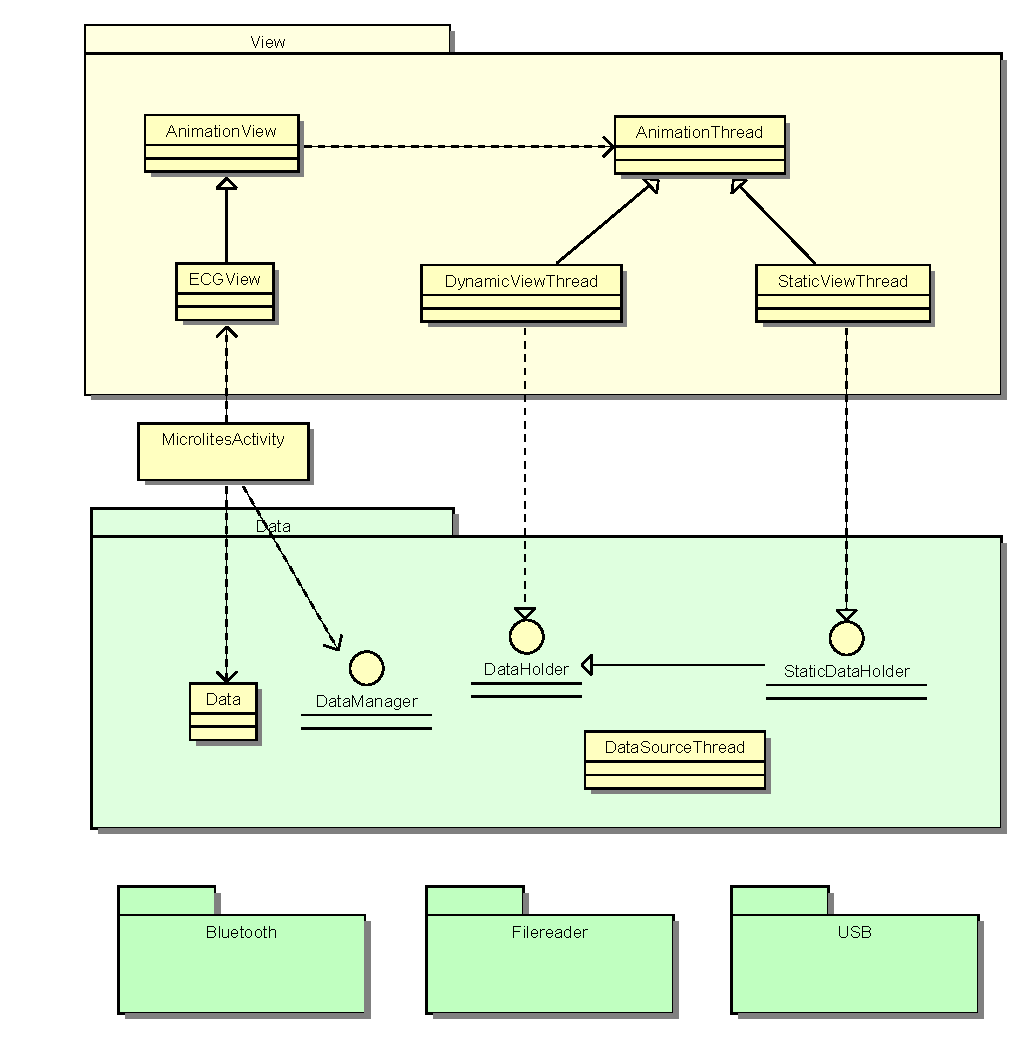
\includegraphics[scale=0.75]{mlts-arch-main}
		\centering
		\caption{Architecture overview}
		\label{fig:arch-global}
		\end{figure}

		At the core level the main Activity, the View package and the Data package are present, as well as three packages (Bluetooth, Filereader, USB) which will be dealt with later. These components provide the basic elements which compose the model over which actual functionality is built, and are to be seen as the tools available for the overlaying software layer which is addressed next.\\

		The main Activity of the application assumes the role of the central coordinator and is responsible for creation and management of area specific managers, application level data and handling of the aforementioned user interfaces stack. It is also responsible, as the application's entry point, of the presentation and behaviour management of the main application menu which gives access to actual functionality, delegating in the specific managers.\\
		
		Of all those tasks, the most important are the initialization and eventual finalization of data visualization flows in collaboration with the appropiate area specific manager. Throughout the process, mainly controlled by the activity, components required for the visualization process are initialized, delegating area specific tasks to the manager. Eventually, the manager assumes the control of the application flow, leaving the activity as a dispatcher of input events.\\

		% Model: Core, domain specific components that require realization in order to work.
		% Model involves: a Manager, a DataSource and a DataHolder (as well as a DataParser) and, if visualization is required, the ECGView and a ViewThread derivate.
		% The model needs to be realized for it to work, the Activity is just an engine running an instance of the model.
		% "It follows a factory pattern, but the factory is the Activity."

		These managers are part of the so-called, in the project terminology, a model; and the activity can be portrayed as the model manager. Conceptually a model is a set of software entities which live in the application and handle the data flow from a given data source towards a data holder, including or not, the visualization of such data. A model contains a Manager which is the entity responsible of the handling of the rest of the model entities. Please note that this model scheme is  specific to the domain of the project and is not a general one\todo{Remove this note? Leave this note?}.

		\begin{figure}[h]
		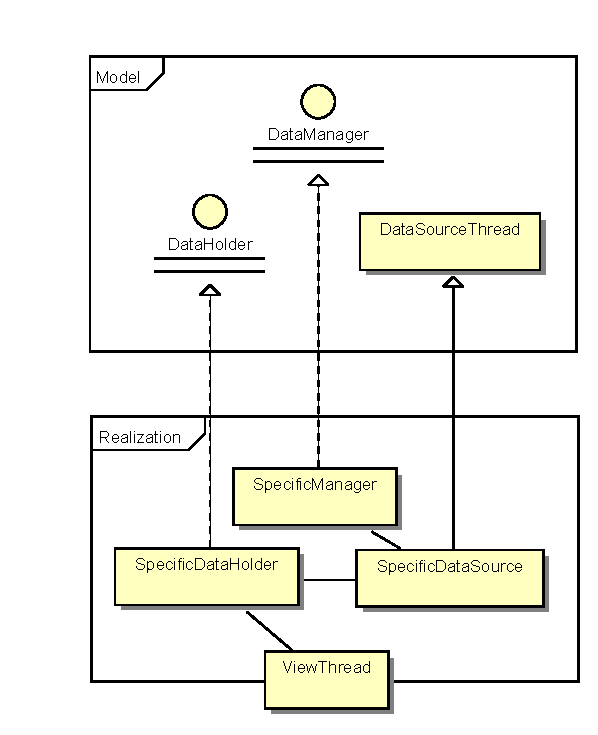
\includegraphics[scale=0.75]{mlts-arch-model}
		\centering
		\caption{Data-flow model realization}
		\label{fig:arch-model}
		\end{figure}

		This conceptual model \todo{Rename model to FlowModel?} scheme is provided by a subset of the classes and interfaces shown in \autoref{fig:arch-global}. For actual functionality building a realization of the model is to be developed, giving actual meaning to the scheme. In the scope of the project four model realizations have been implemented and will be detailed later.\\

		A model realization is composed of implementations of the following elements from the core level exposed before: 1) a Manager, which handles user interaction and required preparations; 2) a DataSource that manages raw data obtention from the actual source, and processing and sending of such data to a 3) DataHolder, which stores and handles the data in any required way and, if data visualization is required 4) an implementation of a view thread.\\

		More detailed approaches to all the concepts exposed in this introduction are built throughout the following subsections.

		\subsection{View Package}
		\begin{comment}
		Realtime rendering required a special, non full common functionality (slide, scroll, ...) providing View derivate: SurfaceView. It provides a bitmap surface where you can draw whatever you want. Derived into AnimationView with employment of AnimationThread for obtaning a good old while(!finished) \{update(); render();\} loop.
		That structure derivates into ECGView which is a domain specific specialization of AnimationVeiw and Dynamic- and StaticViewThread. The later two implement behaviour expected of Dynamic and Static data visualization respectively (more on this on the Data Package)
		Programming style in this area closer to C than to an OOP language in order to maximize performance. (Talk about intolerable initial performance caused by extreme number of new each step and too much relaying on GarbageCollector?)
		\end{comment}

		The set of classes encompassed in the View package (see \autoref{fig:arch-global}) provides both a base rendering architecture in an update-render loop style not initally present in the Android framework and the specialization of such architecture for the specific project domain, i.e. plotting of the electrocardiogram wave and its relevant points.\\

		Regarding rendering Android provides a set of common employed visual elements. These implementations try to simplify the developer's work by giving customizable solutions to common scenarios, such as rendering a list of elements or a drop-down selection object, in a visually pleasing way. All this elements are part of the hierarchy of Android's View class, and implement a composite pattern for rich menu-building.

		The soft real-time rendering imposed by the project restrictions requires a specific View \todo{reference to View in andev?} class derivate: the SurfaceView. This kind of View provides a bitmap surface where pixel-level rendering is allowed. A set of rendering tools is also provided by Android. The architecture developed on top of that view extends the SurfaceView to an AnimationView and delegates the rendering to an AnimationThread. This last entity is the one providing the update-render loop employed for the real-time rendering. The drawback of employing a SurfaceView as the base is that such element doesn't provide common employed functionality as scrolling or zooming.\\

		The actual, domain specific rendering functionality providing threads are implemented employing the aforementioned layer as a base. The precise entities are DynamicViewThread and StaticViewThread, and are referred in this document as implementations of the view thread, even if such class does not exist in the project. This two classes implement the required behaviour for dynamic and static data visualization respectively, and obtain the data to be shown from a data source entity. Such entity is dealt with in the following section. The reason for different entities to exist for static and dynamic rendering is also detailed there.\\

		\subsection{Data Management Package}
		\begin{comment}
		Data class acting as a centralized data storage. Provides app-level synchronization too.
		Different models for static and dynamic data management.
		Dynamic: manages its own data and implements replacemente and discard politics, data is provided by single units. This is so because of the way the data is received and then parsed in real-time.
		Static: obtains a reference to the data location, which is where the actual data manipulation is done. This way huge ammounts of data transfering is avoided (read file can contain lots of megabytes of data which can't be passed at once to the holder). First try was passing the whole array of samples but that was unassumable in real-time.
		DataSourceThread is a receiver by concept, but concrete implementations might require actual communication, that is, data reception \emph{and} data sending. As a developer facility, any DataSourceThread must provide an implementation of a method for writing data into the actual raw data source, expected to act in a similar manner to the one the DataSourceThread does in the inside.
		\end{comment}
		
		This package contains data storage and handling related entities. Differentiation between two types of data managed by the application depending on their purpose is mandatory. On one hand is the application level data, which is specific or non-specific information shared by the whole application. On the other hand is the data received from a source that must be visually presented to the user or stored for later visualization. Providing software tools allowing the modelling that data flow is the key task of this package.\\

		The class Data acts as a centralized application level data storage. It is a singleton and is accesible by every entity in the system. It also provides syncronization methods for correct inter-thread communication.\\

		The rest of the entities of the Data package are employed in the aforementioned model scheme, and specify the expected behaviour of each element involved in a data flow. As indicated before, specialization of this entities is required for the realization of the model.\\

		%\begin{wrapfigure}{l}{0.35\textwidth}
		\begin{figure}[h]
		\begin{center}
	    	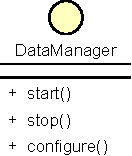
\includegraphics[width=0.20\textwidth]{mlts-ent-datamanager}
  		\end{center}
  		\caption{DataManager interface}
		\end{figure}
		%\end{wrapfigure}


		DataManager is the interface to be implemented by the model controller. It is responsible for the configuring, starting and halting the data flow provided by its controlled entities. It also participates in the process of initialization of the visualization \todo{Link to this process} of a data flow by communicating a DataHolder with the respective DataSourceThread.\\

		A DataSourceThread is a thread which provides data to other entities in the system, generally to a DataHolder. It is a specialization of Thread with functionality to start and stop the flow of data. This data is usually received from an external entity, such as a USB device or a file, and concrete implementations  might require an actual communication between the two, forcing the DataSourceThread to send data to the other end of the connection. Because of that, any specialization of this class must also listen to petitions of writing to its data provider when available.\\

		%\begin{wrapfigure}{l}{0.35\textwidth}
		\begin{figure}[h]
		\begin{center}
	    	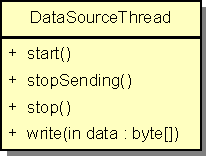
\includegraphics[width=0.3\textwidth]{mlts-ent-datasource}
  		\end{center}
  		\caption{DataSourceThread class}
		\end{figure}
		%\end{wrapfigure}

		The processing of raw data sent by the data providers to the DataSourceThreads is expected to be done in the latter, so the data transfered throughout the application is of a processed nature. To this end the DataParser entity is available\todo{Reference DataParser}.\\

		The expected receiver of the data sent by a DataSourceThread is a DataHolder. This interface provides domain-specific data handling abstract methods and definitions. An implementation of a DataHolder must handle the reception of ECG wave samples, delineation points, synchronization points and heart-beat-rate values.\\

		%\begin{wrapfigure}{l}{0.35\textwidth}
		\begin{figure}[h]
		\begin{center}
	    	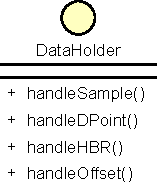
\includegraphics[width=0.20\textwidth]{mlts-ent-dataholder}
  		\end{center}
  		\caption{DataHolder interface}
		\end{figure}
		%\end{wrapfigure}

		The actual way in which that data is employed depends on the concretion of the interface, and might or might not involve visual representation. When visual representation is required, the view thread implementation should also implement the DataHolder interface.\\

		%Dynamic: manages its own data and implements replacemente and discard politics, data is provided by single units. This is so because of the way the data is received and then parsed in real-time.
		%Static: obtains a reference to the data location, which is where the actual data manipulation is done. This way huge ammounts of data transfering is avoided (read file can contain lots of megabytes of data which can't be passed at once to the holder). First try was passing the whole array of samples but that was unassumable in real-time.

		There are two different specifications for the data holders: DataHolder and StaticDataHolder. This is so because of the two modes of operation\todo{Is it clear that there are two modes of operation?} of the application. One is real-time data visualization and the other is log file visualization. The former is called dynamic visualization and the latter static visualization, and the behaviour of their DataHolders is not the same.\\

		Dynamic visualization represents data received in realtime by the DataSourceThread. The DataSourceThread obtains the data from an external entity, processes it and sends it to the DataHolder. This data usually arrives in groups of variable size, and is provided to the DataHolder in single units once processed. In this scenario the DataHolder is the view thread, and handles data however considers optimal. In the implementations developed in this project a fixed amount of data is held and older information is replaced by the new one as it arrives.\\

		Static visualization, on the other hand, involves reading a file, usually megabyte sized. The receiving of big quantities of data in single units by the data holder, as would occur if  the original DataSource specification was employed, could lead to severe slow-downs and application performance would be affected. To avoid such issues, the StaticDataHolder specification is developed.\\

		A StaticDataHolder does not actually hold the data: it delegates that task to its DataSourceThread. The data source will provide the StaticDataHolder with a reference to the actual data. This way big amounts of data transferring is avoided. The inheritance relation between DataHolder and StaticDataHolder is imposed by the architecture, which require a DataHolder to be passed to a DataSourceThread.\\

		\subsection{Utilities Package}
		\begin{comment}
		Contains application level reusable components as two different DataParsers (one for realtime, on for static data which doesn't store what it reads). Also contains the Viewport entity employed as a container of the view parameters. An unused color picker is there (not mention!)
		\end{comment}
		This package contains reusable components providing very specific functionality so they are considered utilities: RealTimeDataParser, StaticDataParser and Viewport.\\

		A data parser is the entity responsible of the processing of the raw data obtained by a DataSource into the domain specific data that the application manages. There are two implementations, one for real-time data reception, RealTimeDataParser, and the other for static data reading, i.e. a log file. The real-time data parser is also responsible of storing the received raw data to a log file.\\

		A data parser is intended to be contained in a DataSourceThread. It receives the bytes of raw data and, upon successful identification of a valid data element, notifies the corresponding DataHolder entity of the arrival. In a theoric, performance-independant model, this behaviour would be incorrect: the data parser would leave the processed data \emph{in} the DataSourceThread, which would then make the transfer of information to the data holder. This kind of implementation is not valid with the soft realtime requirements of the project, as the data source - data parser - data source - data holder flow would be a severe bottle-neck.\\

		The Viewport entity is a container for the visualization area settings. It represents the window in which the data plotting is done, and holds information about size and position of it. It also contains data about the horizontal and vertical scale of the rendering and handles modification of all these parameters. It is employed by the view thread hierarchy.
		
		\subsection{Data Flow Model Realizations}

		Having explained the data flow model scheme and the core level architectural elements employed in its construction, model realizations implemented are detailed next. For each realization, the concretion of each model element will be exposed including particular details of such implementation.

		\subsubsection{Bluetooth Model}
			The Bluetooth \todo{Bluetooth (TM)?} model is a real-time visualization targeted data flow where the actual data provider is a Bluetooth node. As visualization is an objective, this model realization employs a DataManager, a DataSource, a DataHolder and a DynamicViewThread; the latter two being implemented in the same entity. An overview of the realization is shown in \autoref{fig:arch-bt}.\\

			\begin{figure}[h]
			\centering
		    	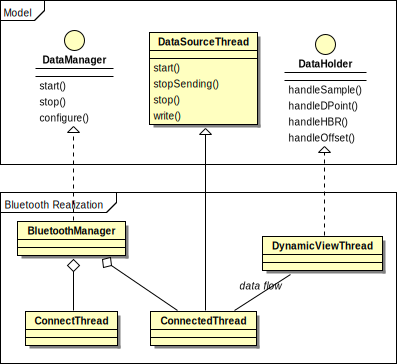
\includegraphics{mlts-arch-bt}
	  		\caption{Bluetooth Model Realization}
			\label{fig:arch-bt}
			\end{figure}

			The specialization of the DataManager is the BluetoothManager. It prompts the user for the device to connect to and handles connection by employing two threads: ConnectThread and ConnectedThread. After discovering the available nodes, it locates the node indicated by the user and launches the ConnectionThread.\\

			This ConnectThread is the thread which actually manages the connection by obtaining its endpoints in the form of a socket. If successful, passes the socket to the manager and finishes its execution. The manager then launches the ConnectedThread, which receives the socket and data flow starts. The reason for employing a thread for establishing the connection is to avoid blocking the application while connecting.\\

			ConnectedThread is the DataSourceThread implementation and contains an entity of DataParser. It receives data sent by the Bluetooth device through the socket, parses it and notifies the DataHolder implementation, which is the DynamicViewThread. The DataParser in DataSourceThread is a RealTimeDataParser and stores the data in a log file while processing.

		\subsubsection{File Reader Model}
			This model realization implements visual representation of ECG data stored in a log file. It is a static view model, in which the user controls what section of the temporal log is shown on-screen, an thus employs an StaticViewThread instead of a dynamic one.\\

			\begin{figure}[h]
			\centering
		    	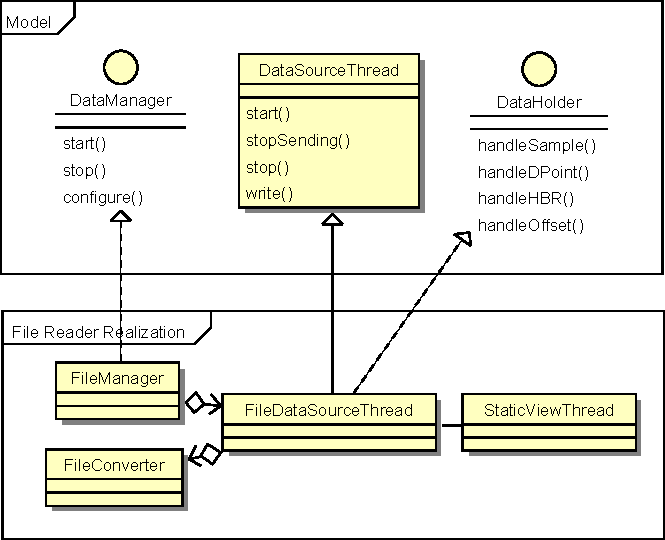
\includegraphics{mlts-arch-log}
	  		\caption{File Reader Model Realization}
			\label{fig:arch-log}
			\end{figure}
		
			The manager in the file reader model is the FileManager class. It presents available log files to the user, handles the seleccion of one, instantiates the file reading thread and connects this with the view thread. When the user finalizes the visualization of the selected log, the FileManager returns to the log selection menu instead of going directly to the main menu. This is an example of the versatility of the aforementioned view stack scheme, which lets specific managers present as many menus to the user as necessary.\\

			FileDataSourceThread is the thread that reads the chosen file and processes its data. It implements both the DataSource and the DataHolder interfaces, so it acts as the emitter and the receiver of the processed data. The view thread obtains a reference to this same data, thus avoiding big amounts of data transferring in the static view model as explained before. This is an example of the flexibility sought by the architecture design.\\

			The FileDataSourceThread, thus, manages data reading, storage and manipulation. The data is read from files with the aid of this package's FileConverter entity. This files can be of big size, so they should not be fully loaded onto memory. A partial load is mandatory in such cases, and the next chunk of data is to be read when the ``visualization window'' approaches. All this management is done by the FileDataSourceThread.\\

			When the view is controlled by the user, i.e. horizontal scroll, the event is passed directly into this thread from the StaticViewThread. FileDataSourceThread then updates the portion of the data to be shown. The updated information is consulted by the view thread in the next rendering step. That way, were further file reading required, it could be done in a transparent-to-view manner.\\

			Data processing is done employing an instance of StaticDataParser in the FileDataSourceThread.\\

			The FileConverter entity provides functionality to transform a given file to a Stream, ArrayList or array of bytes, the latter being the expected input format for the available data parsers.

		\subsubsection{USB Model}
			The USB model manages data reception from an USB device and eventual visual representation for the user. It is a real-time data flow, and thus employs a dynamic view thread. An overview of the model is shown in \autoref{fig:arch-usb}.\\

			\begin{figure}[h]
			\centering
		    	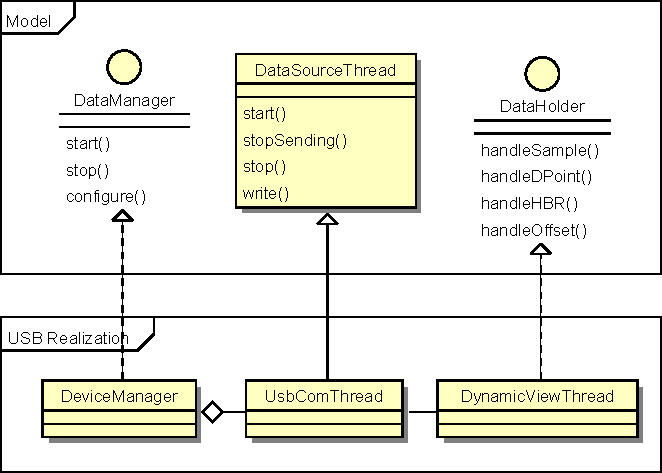
\includegraphics{mlts-arch-usb}
	  		\caption{USB Model Realization}
			\label{fig:arch-usb}
			\end{figure}

			DeviceManager is the realization of the model's Manager. This entity handles connected USB devices enumeration and selection by the user. If only one device is available, connection is directly stablished with it. Differing from the Bluetooth realization implementation, the actual connection to the device is handled by the DeviceManager in a blocking manner. It is so because USB connection resolution takes very little time and the delay is virtually imperceptible for the user.\\

			Once the connection is stablished, the DeviceManager launches a UsbComThread. This thread is the specialization of DataSourceThread and obtains the raw data from the USB device, processes it employing an instance of DynamicDataParser and sends the results to the view thread. This is a DynamicViewThread entity.

		\todo{Extra things here? (see source file) || Diagrams like these would rather be an appendix, could be cited from here}
		\begin{comment}
		\subsection{More things (which I don't know where to include}
			
			\texttt{(These with sequence diagrams and all)}
			Explanation of the visualization initialization procedure, as well as the finalization one.
			Example of a full data flow (e.g. bluetooth)
		\end{comment}

	\section{Implementation Details}

		\begin{comment}
			Potential iterations
			It1. Bluetooth + Architecture prototype
			It2. USB + Log
			It3. Architecture rewriting
			It4. Adding it all and finishing

			For iteration description:
				+ objectives
				+ objectives description
					realization, done?
				+ Use Cases realized
				+ expected and spent time
				+ extra objectives
				+ prologue to next iteration

			Describe risk statuses updates in each iteration?
		\end{comment}

		% Intro
		In this section a detailed description of the development is presented. The evolution of the application architecture and functionality; design, architectural and implementation decisions and explanations of the circumstances in which they were made, as well as the development of the project schedule are exposed in chronological order.\\

		The section is arranged following the five iterations of the project, developing each one by presenting the target objectives and expected deadlines for the iteration, detailing application evolution with emphasis on use case realization and risk suppressing achievements and demonstrating the state of the project as assessed on the reviewing meeting conducted at the end of the iteration.

		% Scheduling
		\subsection{Project Scheduling}
			
			Before diving into the description of the development process an overview of the project schedule % and the reasons for it to be as open as it is
			is mandatory.\\

			As was mentioned in the previous sections, an agile software development methodology has been applied to the project, even if artifacts from more ordered and structured methodologies have been employed to avoid losing focus on the critical aspects of the development.\\
	
			Software development project being dependant on parallel-conducted hardware research, project assets, both personal and development resources, being shared with the hardware research having the former higher priority, and team's lack of formation regarding Android development are some of the factors which lead to the adoption of such a mixed methodology. As they have been already exposed in previous sections, they won't be detailed here.\\ %Consult [X][Y][Z]... for details

			In such an scenario, a fully developed, eight month covering schedule was unfeasible, at least with the imposed time restrictions which didn't allow much time to be spent on planning. The decision was then made to plan only the earlier project iterations, assuring critical functionality identified from use case development to be implemented as soon as possible as well as higher threat involving risk suppression to be realized.\\

			Actual software project development begun October 15, 2011, being the final deadline set on June 15, 2012. That deadline could not be pushed any further, so an estimated deadline was set on May 31, 2012, leaving half a month for further work or recovering from delays, and seven and a half months of development time.\\
		
			Time was needed for the hardware research to start providing results, and no work could be done in the meantime on related application parts. Considering also that even in the most optimistic scenarios no actual work with the 802.15.4 USB receiver couldn't be done until mid February [link to hw planning or something], the schedule had to assume that the first four months of software development would need to cover the implementation of most of the features, leaving the rest of the development time for implementing hardware-related requirements, which couldn't actually be scheduled until hardware research was evaluated.\\

			The adopted schedule dealt with the aforementioned facts by proposing five iterations, from October 15 to May 30, complying with the fifteen days reserved for contingencies. The first three iterations had a duration of two months, the third one a single month, and the remaining one was fifteen days long.\\

			Having the previously developed iOS application as starting point, and being achieving at least the same feature list of that a critical target of the project, the first two iterations were planned so as to realize \textbf{UC1} and \textbf{UC3} which captured requisites expressing such feature list.\\

			The next iterations were just scrapped as no accurate estimation could be done on the state of the project by those dates. Thus, the third iteration was planned to cover the implementation of the remaining features, namely, communication with the 802.15.4 receiver device, the fourth one reserved for polishing the application and the fifth one left for testing and validation. The fourth iteration was to shrink if objectives were achieved quickly to leave more time for validation.\\

			The scheduled distribution of work for each iteration is as follows:\\

			\begin{tabular}{| c | l | l |} % | l | para el hw
				\hline
				It & Dates & Activity \\ \hline
				1 & Oct 15 - Dec 15 & Application base and Bluetooth module\\ \hline
				2 & Dec 15 - Feb 15 & Log module and initial USB module\\ \hline
				3 & Feb 15 - Apr 15 & Final USB implementation \\ \hline
				4 & Apr 15 - May 15 & Polishing \\ \hline
				5 & May 15 - May 30 & Validation \\ \hline
				- & May 30 - Jun 15 & Reserved \\
				\hline
			\end{tabular}\\\\

			Which can be seen as the following expected use case realization dates:\\

			\begin{tabular}{| c | l | l |} % | l | para el hw
				\hline
				It & Dates & Realized Use Case \\ \hline
				1 & Oct 15 - Dec 15 & UC1, UC4 (first version)\\ \hline
				2 & Dec 15 - Feb 15 & UC3, UC2 (first version)\\ \hline
				3 & Feb 15 - Apr 15 & UC2 (final) \\ \hline
				4 & Apr 15 - May 15 & UC4 (final) \\ \hline
				5 & May 15 - May 30 & Validation \\ \hline
				- & May 30 - Jun 15 & Reserved \\
				\hline
			\end{tabular}\\\\

			Throughout the development, as expected, this schedule had to be adapted as the hardware research advanced to assess the arise of difficulties and subsequent changes to its planning. Instead of providing a fixed snapshot of the altered schedule at the end of the project, a detailed description of each iteration is presented next, including modifications to the planning and the motivation for making them.

		\subsection{Iteration 1}

			The main objectives for this first iteration were
			\begin{itemize} 
				\item the instruction of the team on Android development, 
				\item the lay out of an initial version of the application architecture and
				\item the implementation of the Bluetooth receiver module.
			\end{itemize}

			The alloted time for the iteration was of two monts, from October 15 to December 15. During this period the hardware research didn't require much resources [link to hw], so in practical terms the full team was employed in the software project.\\

			In order to minimize risk AR1[quote?link?], the instruction of the team on Android development becomes the key objective for the iteration. Development starts with the implementation of the designed base architecture for the application, so it serves as a powerful learning resource. The notion of that implementation as disposable is not abandoned throughout iteration time and it is always considered as a prototype to evolve or be substituted by a more refined version once team's knowledge of Android increases.\\

			Having the basic architectural framework developed, implementation of the Bluetooth receiver module begins. Special care is put both on design and implementation, as this functionality has to be ready as soon as posible, and little time will be available for reimplementation further in the development.\\

			Testing of both architecture and Bluetooth module is conducted during the whole iteration, specially in the final weeks, so by the end of the iteration Bluetooth module is validated and expected to be stable until the scheduled architectural redesign.\\

			As the Android formation phase takes less time than expected and hardware research doesn't allow advancing into next iteration at the time iteration objectives are achieved, an extra implementation effort is put to begin implementation of UC4. Adjust View Parameters.\\

			In the review meeting for the iteration the following conclusions are obtained:
			\begin{itemize}
				\item Basic architecture implementation is done.
				\item Android is confirmed to be a very comfortable development environment even if non-standard functionality is not that easily achieved. Instruction is planned to continue.
				\item Realization of UC1-\emph{View data from Bluetooth} is finished. Related user interface is not final, but it is functional, and is to be updated on further iterations.
				\item Realization of UC4-\emph{Adjust view parameters} is done in relation to Bluetooth visualization. As remaining modules are developed, further work is to be done in this field.
			\end{itemize}

			\begin{comment}
			Results and adaptation of pre-planned it2
			Risk evolution!?
			\end{comment}
			
		\subsection{Iteration 2}

			The main objectives for the second iteration are
			\begin{itemize} 
				\item the development of the USB communication module and
				\item the implementation of the Log visualization module.
			\end{itemize}

			The hardware reserarch having provided successful results regarding the initial prototypes of the USB accessory, the scheduled USB module implementation for this iteration is mantained, but delayed until further testing can be done in the hardware area.
			In that scenario this iteration begins by the addressing of the implementation of the log visualization module. \todo{This sentence sounds odd, to be fair/kind.}\\

			Module design and implementation are to change little in following iterations to allow the scheduled architecture rewriting to be realized and trying to minimize the possibility of risk PR1. This situation and the fact that a lot of resources are required in the hardware area makes the consecution of this objective fill most part of the iteration time.\\

			Full expected functionality is implemented, including the remaining features from UC4-Adjust view parameters, but validation testing indicates low performance in log visualization caused by big memory requirements. Effort needs to be put into the other iteration objective, so log visualization is halted at this point, scheduling the development of required optimizations for the next iteration.\\

			Having the USB accessory prototype in an usable state, development of the USB communication module begins. At this point the USB accessory could only operate assuming the role of host in the connection, so the disposability of the module is acknowledged. Nevertheless, this implementation is a must if the project goals are to be achieved, as it serves as first-hand instruction regarding USB development in Android. Moreover, if the hardware project is unable to produce an USB slave accessory, with the developed module the project would not have fully failed. Eventually this development has proven being key for the first tests with the actual target hardware platform.\\

			During the implementation of the USB communication module the log writing is improved, so, except for the aforementioned performance optimizations, the log part of the application is finished.\\

			With the basic interface, disposable architecture and fully functional data flow modules, full application functionality is implemented by the end of the iteration, and in the review meeting the following conclusions are obtained:
			\begin{itemize}
				\item Full functionality has been implemented in the application and the product of this iteration is, as expected, the first prototype of the application.
				\item Realization of UC2-\emph{View data from USB Receiver} is realized until hardware research advances. Current implementation can act as the actual version of the use case realization if hardware research is not fulfilled.
				\item Realization of UC4-\emph{Adjust view parameters} is now finished. All required view controls are implemented.
				\item Risk PR1-\emph{Application functionality inferior to that featured by existing iOS application} is marked as surpassed, as key functionality is implemented.
				\item Risk MR1-\emph{Mobile device unsuitable for target functionality} is identified to require further monitorization and is unfolded into risks AR2 and AR3.
				\item Risk AR2-\emph{Android providing subpar performance when handling required data} is confirmed to occur and is to be solved in the next iteration.
			\end{itemize}

			\begin{comment}
			Log writing improved.
			USB module done as USB device, valid for arduino and first msp tests
			Log reading implemented, scrolling and such. Tests results indicate low performance, huge memory requirements.
			With the basic interface, first Prototype with (except usb host == 802.15.4) full functionality implemented. That nice and all. Shown to masters and feedback applied.
			On time ?
			
			Took a loong break here for hardware development
			% Here ends electroiltes
			\end{comment}

		\subsection{Iteration 3}
			% This is microlites
			\begin{comment}
			This is the first just-drafted iteration. Starting from the fully functional prototype, architectural and performance fixes were mandatory. Also, given the positive state of the hw research scheduling was done for the rest of the iterations.

			The main objectives for this third iteration are
			\begin{itemize} 
				\todo{Remove leading ``the's'' to improve readability?}
				\item the redesign of the application architecture, 
				\item the achievement of required performance in data management and
				\item the scheduling of the rest of the project time.
			\end{itemize}

			~(Scheduling seems strange as an objective)~

			Architecture redesigned targeting easy adaptation and versatility inside the scope of the application. Redesigned visualization initialization flow.
			Performance increased significantly and memory usage reduced THROUGHOUTLY in realtime view.
			Fixes in modules according to new architecture.
			Talk about scheduling??
			\end{comment}

			This is the first just-drafted iteration of the original scheduling. Taking the prototype obtained in the previous iteration, architectural redesign and performance optimizations are mandatory. Performance optimizations are  identified to be required in two areas: data management and data rendering. Only data management related optimizations are addressed in this iteration.\\

			Iteration objectives are as follow:
			\begin{itemize} 
				\item redesign of the application architecture, 
				\item achievement of required performance on data management, and
				\item scheduling of the rest of the project time.
			\end{itemize}

			The main lack of the basic architecture of the protoype is that it was implemented to serve as a quick prototyping base for the data flow modules. The instruction and knowledge about the platform and the way of operation obtained in the previous iterations are applied in the new architecture design.\\

			This design is done targeting easy inclusion of new data flow modules allowing them to employ their own user interfaces, while providing core level software entities for building those modules. This process produces the architecture as exposed in \autoref{sec:sw-arch}.\\

			A detailed analysis is conducted on the data management related operations in the application, identifying the ubiquitous application of the object oriented model proposed by Java added to the subpar efficiency of the Garbage Collector \todo{Reference something? Could be added a screenshot from that Eclipse performance analysis tool?} as the main cause of performance loss. The alteration of the programming paradigm and the employment of as basic software entities as possible, substituting classes\todo{Perhaps ``avoiding continuous object instantiation'' better?} used to, e.g. contain the four parameters of a wave delineation point, by more basic structures, like the same four numbers stored independently, proved to be the most effective methods of avoiding low performance.\\

			Following such lines of operation, performance regarding data management is utterly improved on spite of a less developer-friendly programming environment. During this process the data flow modules (Bluetooth, USB and Log Viewer) are also tweaked.\\

			The positive results obtained both in the software and hardware areas allow a solid review of the project schedule. The decision is made to keep the division of the remaining project time in two iterations, leaving the last, fifteen days period for unforseen difficulties. Of the two iterations, the first is to be devoted to implementation of the USB host communication as hardware project estimates completion of a first prototype halfway the iteration; and the second, and last, iteration is planned to be employed in final testing and validation of the application against hardware prototype.\\

			The following conclusions are obtained from this iteration's reviewing meeting:
			\begin{itemize}
				\item The architecture of the application is finished and validated.
				\item User interface is yet to be final and is to be addressed at the following iteration.
				\item Identified solutions for performance issues are to be applied in the rendering area.
				\item Risk AR1-\emph{Lack of instruction on Android development delays workflow} is marked as surpassed as the team feels comfortable enough with Android development.
				\item Risk AR3-\emph{Android rendering capabilities unable to handle required data} probability is increased to Moderate and is to be addressed in the next iteration.
				\item Risk HR2-\emph{802.15.4 receiver device unfeasibe} probability is reduced to Low as hardware research is providing positive results.
			\end{itemize}

		\subsection{Iteration 4}
			\begin{comment}
			Final implementation iteration. Final performance increasing fixes and user interface implementation, as well as user-friendliness globally increased.

			USB Host here!

			The main objectives for this third iteration were
			\begin{itemize} 
				\item the implementation of USB host communication,
				\item the achievement of required performance in rendering and, 
				\item the implementation of user-friendly interfaces.
			\end{itemize}

			This ends the implementation phase, user-friendlyness could be better but what gives. 
			Performance left 50-50 because it was already ok (30fps not 60fps).
			One iteration left, devoted to testing.
			\end{comment}

			This iteration is scheduled to be the last implementation iteration, and it's objectives are:
			\begin{itemize} 
				\item the implementation of USB host communication,
				\item the achievement of required performance in rendering and, 
				\item the implementation of actual user interfaces.
			\end{itemize}

			The USB slave accessory prototype is produced on time by the hardware project, and implementation of the actual USB communication assuming the Android device the host role is done in very short time, leaving room for consecution of the rest of the iteration objectives and following validation.\\

			Employment of the identified working solutions for performance issues in the rendering area doesn't provide the expected results, and further research is required. The bottle-neck in the rendering process is indentified to be the context change required by the rendering tools provided by Android. Meticulous research on Android developer resources provides no other solution than minimizing the number of calls to the rendering methods each step. Emphasis is put to the realization of this task, but to no avail.\\

			The problem is the big amount of data required to be drawn each rendering step. A mechanism is developed to minimize the number of lines drawn by joining similar valued wave points, and the performance is improved, but not at the desired level. Nevertheless further work in this area is postponed as the achieved performance lies in the range required by the non-functional requirements of the project.\\

			Implementation of the actual user interfaces to be employed in the application is addressed next. The design of these has been done throughout the last two iterations. The implementation process takes more time than expected as	Android user interface framework is quite specific, and requires adequation to certain rules that have to be studied beforehand.\\

			The remaining time of the iteration is devoted to testing and validation of the application, which has reached a near final state. Conclussions from the review meeting follow:
			\begin{itemize}
				\item The Android application is finished and pending validation with the actual USB receiver device.
				\item The application's user interface is in a final state, but were changes required they could be easily implemented as the UI is isolated from the data flow part.
				\item Performance regarding rendering is not optimal, but it is in the range defined by the requisites.
				\item Until validation can begin, the full team can be employed in the hardware project.
				\item Risk HR2-\emph{802.15.4 receiver device unfeasible} is marked as surpassed as the viability of the receiver has been proved by the hardware research.
			\end{itemize}

		\subsection{Final Validation}
			The final effort in this software project extends over the allotted time for both the fifth iteration and the reserved final period. It is fully devoted to testing and validation of both the application and the receiver device. Even if the initial schedule assigned only the fifth iteration to this process, delays on the hardware project \todo{reference hw chapter} force the elongation of the testing phase.

			The objectives for this period are:
			\begin{itemize}
				\item exhaustive testing of the Android application,
				\item validation of the application, the receiver and the delineator node acting as a whole, and
				\item the obtention of the final version of the system by implementing the required amendments identified by the testing procedure.
			\end{itemize}

			Software related testing is conducted throughout all this final step causing minor fixes to be done to the application. No relevant software related issues arise during the testing or the validation phases.\\

			Risk HR1-\emph{802.15.4 receiver device delayed} occurrence is the cause of the elongation of the validation iteration, but has no actual effect on the software project. Even when the receiver is completed \todo{Maybe in a prototype stage, still unknown at Jun, 8} the risk tracking is continued until validation concludes, were hardware complications to arise during the process.\\

			The final, review meeting conclusions are as follow:
			\begin{itemize}
				\item Risk HR1 is marked as surpassed.
				\item The Android application is successfully validated and, thus, completed.
			\end{itemize}
			
	\section{Closure}

	\chapter{Results}
\label{cha:results}

	\section{Final state}
	\label{sec:end-state}
	
		% Describes the fulfillment of this project.

		\todo{Describe battery usage, size requirements actual data}
		% The production of a fully functional, low cost and low sized ECG monitoring system which employs an Android device as the user interface, and it's USB 802.15.4 receiver is completed.\\

		The production of the fully functional, low energy requiring, low sized ECG monitoring system employing an Android device as the user interface and 802.15.4 as the wireless data transferring protocol has been achieved. The system provides all the required functionality: real-time ECG wave data visualization both from 802.15.4 and Bluetooth nodes and storing of the received data in log files for afterwards visualization of these, as well as visualization parameters configuration. The system is, then, a more energy efficient and accessible version of the one produced by the Complutense University of Madrid and the École Polytechnique Fédérale de Lausanne, which is the primary objective of the project.\\

		This achievement is made thanks to the successful outcome of both the hardware research and the software development processes in which the project has been divided. Each of them requiring the employment of specific methodologies and techniques, but being, as they were, highly dependent one on the other only complicated the prediction of the outcome of them both. Thanks to the flexible scheduling conducted for each one, which considered the potential eventualities to arise in the other and focused in allowing rescheduling when necessary, this uncertainty has been correctly managed, leading to the current, successfully finalized state of the project.\\
		
		% HW: The goal of an external 802.15.4 receiver device is fulfilled. Employing it the system is able to render ECG data emitted by a delineator node. Bluetooth is also available, as well as log saving and further reading.\\
		% No olvidar hablar de modificaciones al shimmer!
		Regarding the hardware research part, the main goal pursued was the production of the 802.15.4 USB receiver device for Android systems. This device has successfully evolved from the early stages of development where a prototyping board was employed to a custom developed printed circuit board, which, if has not been produced, is completely designed and validated\todo{Not yet, but soon}.\\

		% Concrete results: X x Y x Z sized device consuming W1 watts of power (actual data, please) which compared to Bluetooth consumption (W2 watts, ...) is pretty low cost, all of this powered by the Android device, and the receiver being plug and play no installation procedure is required.\\
		The prototype board's \todo{Substitute these for the PCB ones if available}dimensions are 7.25 x 6.35 x 3.5 cm, and it requires 3.3V for correct operation, being usable with at least 3.0V. Its USB capability allows for it to be connected to any HID compliant system, and has been successfully employed as an 802.15.4 receiver both in Android devices and Windows based personal computers.\\

		In respect of the Android application, the software development project has produced an Android application providing all required functionality, namely visualization of ECG data from Bluetooth and USB nodes, log saving and reading, and view controlling capabilities, designed and implemented in a robust, expandable manner. Moreover, the application provides a domain-specific framework for the inclusion of new data sources (like Wi-Fi or Near Field Connection) or different source data specifications.\\

		The application presents simple, easy to use user interfaces and very specific functionality, which added to the following of Android proposed application design best-practices smooth the learning curve and allow out of the box usage of the software part of the system. Due to the expansion capabilities of the system, new user interfaces or dialogs can also be added with ease.\\
	
	\section{Potential additions and expansions}
	\label{sec:end-further}
		\begin{comment}
		Potential additions are to target the software frontend application. The developed Android application is a (domain specific) general purpose monitoring frontend that should provide a solid framework for further developments.\\

		Professional multipatient monitoring could come in two flavours:\\

		Visual-less multipatient monitoring in which a computer receives data from a variable number of wireless delineation nodes, e.g. employing the 802.15.4 receiver, storing it and acting as a server, or directly sending the log files to the actual server. The Android device would then download the log from the server and the own frontend application developed in the scope of this project could be used as the visualization device.\\

		The other option is simultaneous multipatient monitorization in an Android device. The monitorization application on the device would allow switching between patient ECG wave visualization while logging all received data, which could then be uploaded to a server.\\

		(Both of these expansions could find an employment in acutal medical environment.)


		More improvements can include the implementation of more detailed log navigation functionality, including information about the actual recording time and searching of specific time moments.
		Inclusion of event data into the log (like body weakness sensation or feeling of dizziness) could also be useful.
		(This two are for personal monitorization and inhome healthcare)\\

		Message sending when certain events occur (low or high hbr or arrythmia detection), text message, email, even a phone call could help constant monitorization requiring people. GPS information could be included in the message for quick localization of the affected person by the healthcare personal.

		% Comentar también como trabajo futuro los requisitos que plantea Marian
		\end{comment}

		Although every initially planned objective has been fulfilled, in addition to several of them which
		were added during the development, there is still room for improvements and features which were
		not considered or left out of scope, since the developed application is not considered as a specific
		product itself, but a framework for further developments. These improvements can be classified according 
		to the period planned for their implementation:

		\begin{itemize}
			\item \textbf{Short-term:} the following features specifically target personal use. Considering
				the user is to monitor his/her own vital signs, the next additions are thought to be useful:

				\begin{itemize}
					\item \emph{Event Tagging}\\
						Assuming the user is feeling funny or pain, it may be quite interesting for him/her
						to be able to annotate such an event with later revision purposes, either by
						him/herself or medical staff. Furthermore, the capability of marking down one peculiar
						result about the ECG delineation can also be useful.\\

						In this way, making use of the tactile interface the Android tablet features, this
						activity can be done by simply touching the relevant event or result. Next, the moment
						which that points refers is logged and a comment may be added to the annotation.\\

					\item \emph{Temporal Meta-Data}\\
						In the same conditions described in the previous item, it is possible that the user
						had felt a particular sensation in a certain moment, yet he/she was unable to mark it.
						Moreover, maybe the annotation was done and it is required to directly jump to that
						certain time.\\

						In order to ease these tasks, time-related data is to be added so that a precise
						moment of the monitoring can be directly found. In this way, the user can input
						the desired date so that the application shows what was happening at that moment.
						In addition, markers from previous annotations would also appear for quickly accessing
						to relevant events.\\

					\item \emph{Voice Commands}\\
						Due to the particular health condition of the user, or just because he/she is busy,
						direct interaction with the monitoring Android device is likely to be impossible. If
						situations like these are to happen, letting users interact with the system through
						their own voice may ease the aforementioned tasks.\\

						Fortunately, Android provides speech recognition support throughout its specific API,
						so this feature could be added without developing the whole voice recognition framework.\\

					\item \emph{Automatic Warnings}\\
						Regarding the user's health condition or unavailability again, automatic message sending
						with ECG data in case of relevant happenings were detected would mean a seamless way to
						warn the user, relatives or qualified staff if needed. In the same direction, multiple
						alternatives would be presented such as emails with GPS location attachments or direct
						automatic voice calls to complement this feature.

				\end{itemize}

				All these features come from a potential project proposed by a specific individual, which, being affected of a certain cardiovascular disease and considering the goals and results of this specific project, has shown interest in further specialization of the developed system for it's particular needs. This private enterprise is yet to be started, but the inception phase has already begun, and is seeking funding. The team of the current project is offering consulting on the viability of the requirements of the project, and testing has been conducted of the already available system with the interested individual.\\

			\item \textbf{Long-term:} this features are mainly ideas which would grant the system with much 
				richer capabilities and new potential, though it would require of a greater amount of time
				along with specific planning and dedication.\\

				On the one hand, the application can be focused towards professional multipatient monitoring,
				which could be developed in at least two alternative ways:

				\begin{itemize}
					\item Since the developed 802.15.4 USB receiver is also compatible with HID-compliant
						devices, particularly computers, multipatient monitoring could be uploaded to a
						devoted server from a variable number of wireless delineaton nodes, omitting the 
						displaying service the Android application provides. Once the data is uploaded,
						the Android device could connect with the mentioned server and download the information
						right from the developed application. Then, the Android tablet would act as usual
						as frontend of the monitoring process, displaying the downloaded data.

					\item Taking into account the relatively big display a tablet device provides, this
						multipatient monitoring paradigm could be directly implemented into the Android 
						device by extending the application's functionality. Among this new functionalities
						there would be switching between ECG wave visualizations of different patients,
						simultaneous logging and server uploading as well.
				\end{itemize}

				On the other hand, regarding self-monitoring, the system can be adapted to be applied to 
				specific domains which impose additional time or resource restrictions.
				Specifically the director of the Embedded Systems Laboratory at the EPFL, where the delineator 
				node employed in this project was produced in the aforementioned collaboration with the UCM, 
				has shown interest in the application of the system low power requirements in a specific project
				the EPFL is collaborating with: Solar Impulse\cite{solarflight}.\\

				This particular project tries to achieve a flight around the world employing no fuel, just the
				energy collected from the sun. The airplane used in the project allows only for the pilot to be
				in the cockpit throughout the flight, and, thus, he/she is required to be constantly monitorized.
				Among others, ECG monitorization is required, at is, at the time, being provided by the EPFL and
				UCM monitoring project with the already exposed battery implications of the employment of 
				Bluetooth as the wireless	technology.\\

				Considering that the space in the cockpit is very reduced, and the amount of wires, sensors and
				other instruments that are present, any operation is to be done with special care and only when
				absolutely needed. Concretely, the swapping of a battery-exhausted delineator node for another,
				fully-charged one, to allow the recharging of the first, is a complex procedure as the body
				sensor network wires have to be unplugged from one node and plugged into the other. Moreover,
				while this procedure is being performed ECG monitorization is interrupted.\\

				Reducing the battery consumption of the delineator node is then, a must, and can be achieved by
				the employment of 802.15.4 as the wireless communication protocol. Because of that, the results
				obtained in this project can of great use to the Solar Impulse project.\\
				
				% For instance, adapting the whole system to be used
				% in the cockpit of a solar flight, which represents a special environment with particular
				% requirements, though would benefit from the longer battery life this system provides.
		\end{itemize}
	
	\section{Findings}
	\label{sec:end-findings}

		Development:
		
		Employment of Android for this real-time thingamagigs is not the best thing ever as, even if the devices have high computational power, the restrictions imposed by the operating system hardens the task quite a lot. In that scenario a custom display device would allow finer, prettier visualization of the data, BUT of course the benefits of employing Android like 1. it's already developed duh 2. simplicity of development of visually rich apps and, specially, 3. high availability of the devices which reduces the amount of devices carried, compensate for every drawback it may have. So, asuming some limitations in the display applications (which already can eventually or will be able to be overcome) the selection of Android as a platform has been awesomely great.

		Regarding the process of a project such as this that spawn various subprojects with different characteristics and highly related one on the other, the employment of a flexible schedule, a detailed risk management procedure and focusing a lot on the current objective and it's deadline is critical for a successful outcome.

		Results:

		Ideas: importance of monitorization systems for cardiovascular diseases affected people. Great potential of development in this area. Low cost, low sized, user focused designed, an thus, comfortable application system development is a ineherntly good goal, as are of great help for CVD affected people.

		In this line, 802.15.4 as a low energy requiring wireless protocol significantly reduce the need of monitorization interruption due to battery recharging procedures, which seems like a small thing but is extra nice for minimizing the impact in the life style of the affected people. Also, employment of Android instead of iOS allows things like letting the application work in background while doing other things, shall not be interrupted by an incoming call and such. Also seem like small things but hell if you have to cope with them in day after day.

		Interesting: Marian is interested in the project for personal monitorization, David Atienza (EPFL's ESL \& UCM) is highly interested in the lower energy costs this project has achieved. Also, Solar Flight.


	% Anexos
	\begin{appendices}
		\renewcommand{\setthesection}{\Alph{section}}	% Numeramos con letras
		\appendix
		\appendixpage
		\chapter{Budget Analysis}
\label{ch:budget}

\newcommand*\cleartoleftpage{%
  \clearpage
  \ifodd\value{page}\hbox{}\newpage\fi
}

	Throughout this appendix the project budget analysis is conducted, by detailed specification of both time and resource cost.\\

	The project division in atomic tasks and the scheduling of these is exposed in the first section, in order to justify the cost in engineer hours. The tasks have been given sufficiently explicit names, and have been divided regarding the development iteration they belong to. The Gantt chart ilustrating the project schedule is presented next. Both the hardware and the software subprojects are presented together in it in order to achieve a finer understanding of the project progression.\\

	Once the project scheduling has been exposed, the next section presents the asset cost analysis for the project.\\
	
	\section{Project tasks and scheduling}
	\label{sec:sched}

		\subsection{Hardware project tasks}
		\begin{tabular}{| c | p{6cm} | l | l |} % | l | para el hw
		\hline
			T1.1.1 & Acquire a suitable Android device prototyping environment & 15/10/2011 & 16/11/2011\\ \hline
			T1.1.2 & Manage correct communication between Android and a prototype 		device & 17/11/2011 & 11/12/2011\\ \hline
			T1.1.3 & Develop an application emulating desired behaviour & 12/12/2011 & 19/12/2011\\ \hline
H1 & Arduino for Android USB device Communication & - & 19/12/2011\\ \hline
		\end{tabular}\\\\

		\begin{tabular}{| c | p{6cm} | l | l |} % | l | para el hw
		\hline
			T1.2.1 & Supply MSP430 with USB protocol application functionality & 20/12/2011 & 04/01/2012\\ \hline
			T1.2.2 & Research Android USB protocol related functionality & 05/01/2012 & 19/02/2012\\ \hline
			T1.2.3 & Make Android OS recognize MSP430 when plugged	 & 20/02/2012 & 22/02/2012\\ \hline
T1.2.4 & Manage communication between Android and MSP430 via USB & 23/02/2012 & 07/03/2012\\ \hline
			H2 & MSP430 for Android USB Host Comunication & - & 08/03/2012\\ \hline
		\end{tabular}\\\\

		\begin{tabular}{| c | p{6cm} | l | l |} % | l | para el hw
		\hline
T1.3.1 & Check the proper working of FreeRTOS with the new microcontroller & 09/03/2012 & 13/03/2012\\ \hline
T1.3.2 & Validate the feasibility of the usage of USB API along with FreeRTOS in MSP430 & 14/03/2012 & 23/03/2012\\ \hline
T1.3.3 & Correctly integrate USB API into FreeRTOS & - & 31/03/2012\\ \hline

T1.3.4 & Manage USB data sending in FreeRTOS & 31/03/2012 & 02/04/2012\\ \hline
H3 & USB in FreeRTOS & - & 02/04/2012\\ \hline
\end{tabular}\\\\

\begin{tabular}{| c | p{6cm} | l | l |} % | l | para el hw
\hline
		T1.4.1 & Validate current implementation of 802.15.4 in FreeRTOS in MSP430 testing board & 03/04/2012 & 18/04/2012\\ \hline
		T1.4.2 & Manage connection to the CC2420 radio module to target MSP430 device & 19/04/2012 & 21/04/2012\\ \hline
		T1.4.3 & Port implementation of 802.15.4 to target MSP430 device & 22/04/2012 & 28/04/2012\\ \hline
		T1.4.4 & Prepare implementation of 802.15.4 for actual usage & 28/04/2012 & 09/05/2012\\ \hline
		H4 & 802.15.4 in FreeRTOS & - & 09/05/2012\\
		\hline
		\end{tabular}\\\\

		\begin{tabular}{| c | p{6cm} | l | l |} % | l | para el hw
		\hline
T1.5.1 & Assess conflict-free coexistence of current implementation of both USB and 802.15.4 modules in MSP430 & 10/05/2012 & 16/05/2012\\ \hline
T1.5.2 & Manage sending data received from 802.15.4 via USB & 17/05/2012 & 25/05/2012\\ \hline
H5 & 802.15.4 \& USB coexistence under FreeRTOS & - & 25/05/2012\\ \hline
		\end{tabular}\\\\

		\begin{tabular}{| c | p{6cm} | l | l |} % | l | para el hw
		\hline
T1.6.1 & Exhaustive analysis of the reference board & 10/05/2012 & 21/05/2012\\ \hline
T1.6.2 & Capture of the board schematic & 21/05/2012 & 14/06/2012\\ \hline
T1.6.3 & Design and routing of the actual PCB & 15/06/2012 & 21/06/2012\\ \hline
H6 & MSP430 based device design & - & 21/06/2012\\ \hline
		\end{tabular}\\\\

		\begin{tabular}{| c | p{6cm} | l | l |} % | l | para el hw
		\hline
T1.7.1 & Validate the final version of the receiver device & 26/05/2012 & 16/06/2012\\ \hline
T1.7.2 & Fix possible errors & N/A & N/A \\ \hline
H7 & Final Validation and Release Candidate Version Development & - & 16/06/2012\\
		\hline
		\end{tabular}\\\\

		\newpage
		\subsection{Software project tasks}

		\begin{tabular}{| c | p{6cm} | l | l |} % | l | para el hw
		\hline
IT1 & Complete UC1 & 15/10/2011 & 15/12/2011\\ \hline
   T2.1.1 & Instruction of the team on Android development & 16/10/2011 & 07/11/2011\\ \hline
   T2.1.2 & Lay out of an initial version of the application architecture & 06/11/2011 & 19/11/2011\\ 
   T2.1.3 & Implementation of the Bluetooth receiver module & 14/11/2011 & 03/12/2011\\ \hline
		\end{tabular}\\\\

		\begin{tabular}{| c | p{6cm} | l | l |} % | l | para el hw
		\hline
IT2 & Complete UC4, UC3 & 15/12/2011 & 04/02/2012\\ \hline
   T2.2.1 & Development of the USB communication module & 05/01/2012 & 20/01/2012\\ \hline
   T2.2.2 & Implementation of the Log visualization module & 15/12/2011 & 28/01/2012\\ \hline
		\end{tabular}\\\\

		\begin{tabular}{| c | p{6cm} | l | l |} % | l | para el hw
		\hline
IT3 & Complete Redesign & 15/02/2012 & 15/04/2012\\ \hline
   T2.3.1 & Redesign of the application architecture & 16/02/2012 & 12/03/2012\\ \hline
   T2.3.2 & Achievement of required performance on data management & 13/03/2012 & 28/03/2012\\ \hline
   T2.3.3 & Scheduling of the rest of the project time & 28/03/2012 & 05/04/2012\\
		\hline
		\end{tabular}\\\\

		\begin{tabular}{| c | p{6cm} | l | l |} % | l | para el hw
		\hline
IT4 & Complete UC2 & 12/04/2012 & 11/05/2012\\ \hline
   T2.4.1 & Implementation of USB host communication & 16/04/2012 & 26/04/2012\\ \hline
   T2.4.2 & Achievement of required performance in rendering & 22/04/2012 & 07/05/2012\\ \hline
   T2.4.3 & Implementation of actual user interfaces & 28/04/2012 & 11/05/2012\\
		\hline
		\end{tabular}\\\\

		\begin{tabular}{| c | p{6cm} | l | l |} % | l | para el hw
		\hline
IT5 & Final Validation & 15/05/2012 & 22/06/2012\\ \hline
   T2.5.1 & Exhaustive testing of the Android application & 15/05/2012 & 22/06/2012\\ \hline
   T2.5.2 & Validation of the application, the receiver and the delineator node acting as a whole & 26/05/2012 & 22/06/2012\\ \hline
   T2.5.3 & Obtention of the final version of the system by implementing the required amendments identified by the testing procedure. & 21/05/2012 & 17/06/2012\\
		\hline
		\end{tabular}\\\\

	\cleartoleftpage
	\label{sec:gantt}
	% \begin{figure}[h]
		% \centering
	    	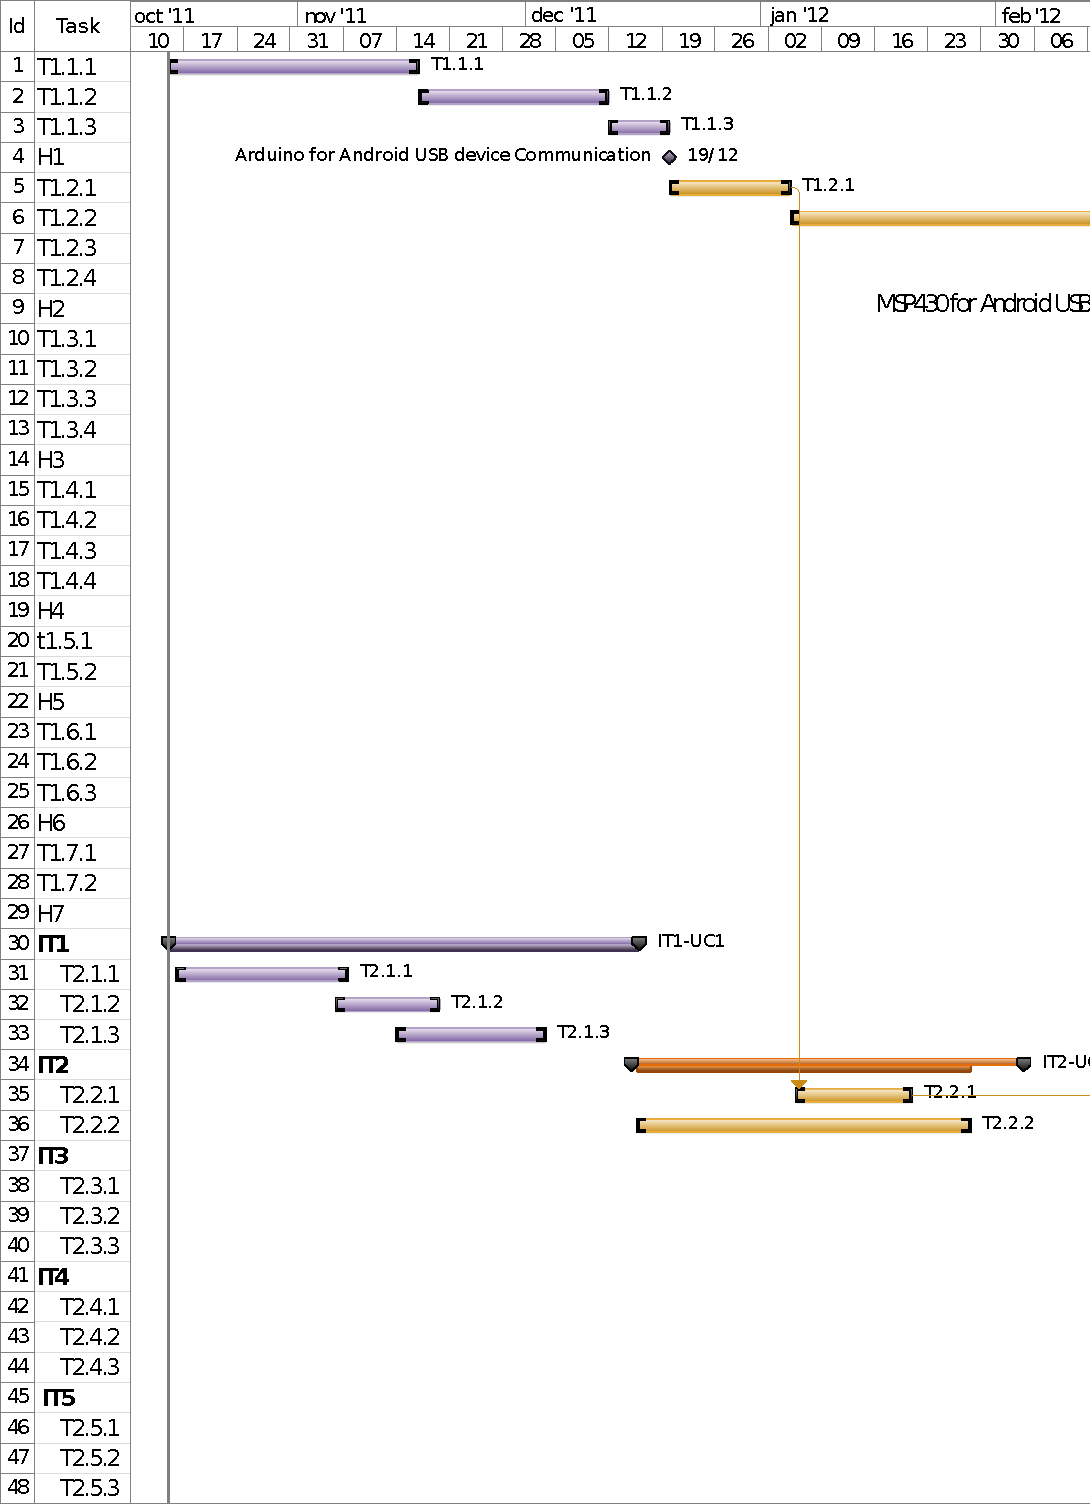
\includegraphics[width=\textwidth]{gantt-l}
		% \label{fig:gantL}
	% \end{figure}
	% \begin{figure}[h]
	 	% \centering
	    	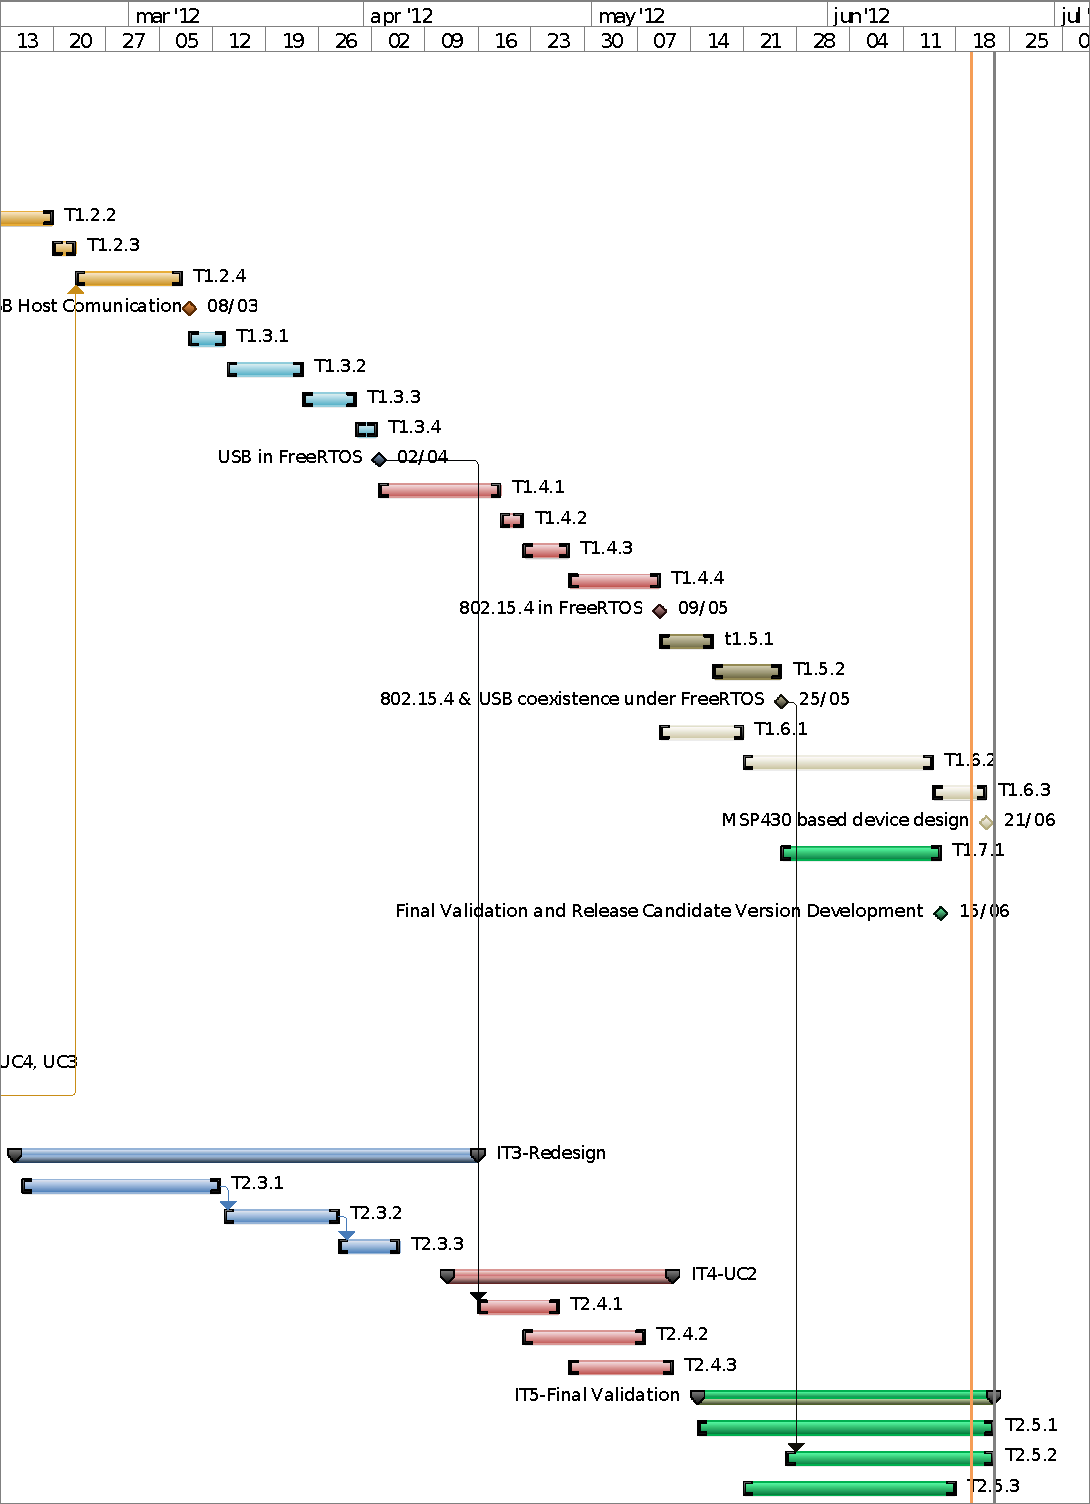
\includegraphics[width=\textwidth]{gantt-r}
		% \label{fig:gantR}
	% \end{figure}
\newpage
\section{Asset cost}
\label{sec:cost}
	% A partir de la planificación anterior, que es la real del proyecto, y considerando que hubo en total cerca de dos meses de vacaciones, podemos considerar que este proyecto tiene una duración de 7 meses con 3 personas trabajando a media jornada. Tipicamente el salario de un ingeniero trabajando en este campo sería de unos 35 euros la hora. Por lo que el coste de un ingeniero durante 7 meses a media jornada sería 35euros/hora * 4 horas/dia * 22 dias/mes * 7 meses = 21560\\
	The total asset cost of the project is presented next, considering the following assumptions:
	\begin{itemize}
		\item The project has been developed through seven months after deducting two months of recess.
		\item Three engineers have been employed halftime through the whole project.
		\item A halftime workday is considered to be of four hours.
		\item The engineer per hour cost considered is 35{\small \euro} per hour.
		\item The ECG delineator node technology is donated and thus is not reflected in the price.
	\end{itemize}

	The cost of a single engineer employed halftime throughout the seven months is of 35{\small \euro}/hour $\times$ 4 hours/day $\times$ 22 days/month $\times$ 7 months = 21560{\small \euro}.\\

	% Este coste, unido al de los productos que habría habido que adquirir si no hubiera habido nada en el lugar donde se realizase el proyecto nos dan el coste total del proyecto:\\
	The breakdown of the cost of the assets of the project is now exposed.\\

\begin{tabular}{| p{5cm} |l | l | l |} 
\hline
   Name & Number& Price per unit & Total ({\small \euro})\\ \hline
   Motorola Xoom - Wifi & 1 & 399 & 399\\ \hline
   Google ADK & 1 & 70.80 & 70.80\\ \hline
   Exp430F5438 + MSP430F5438A & 1 & 117.89 & 117.89\\ \hline
   TS430PZ100USB + 2xMSP430F6638 & 1 & 60 & 60\\ \hline
   CC2420 & 1 & 4 & 4\\ \hline
   Prototype & 1 & 38.60 & 38.60\\ \hline
   Final product & 1 & 42.229 & 42.229\\ \hline
   Engineer & 3 & 21560 & 64680\\ \hline
   Total & & & 65392.13\\ \hline
\end{tabular}\\\\

	The total cost of the development of the project rises to 65392.13{\small \euro}. 

\chapter{Product Cost}
\label{ch:cost}

	% El coste de fabricar un dispositivo de manera individual, que es lo que se ha hecho durante el proyecto es el siguiente:\\
	The cost of the production of both a single unit of the final board and an estimated mass production in batches of 10000 (ten thousand) units is as follows.\\

	In this project a single unit of the board has been produced, with the following, exact cost.\\

\begin{tabular}{| c |l | l | l | l |} 
	\hline
		Name & Reference & Number & Price per unit & Total price\\ \hline
		SMT & 1022311 & 2 & 1.96 & 3.92\\ \hline
		Resistor & 1738981 & 2 & 0.062 & 0.124\\ \hline
		LED & 1699413 & 1 & 0.28 & 0.28\\ \hline
		Capacitor & 1833863 & 6 & 0.03 & 0.18\\ \hline
		Capacitor & 1740650 & 2 & 0.154 & 0.308\\ \hline
		Capacitor & 499110 & 2 & 0.114 & 0.228\\ \hline
		Resistor & 1469918 & 1 & 0.038 & 0.038\\ \hline
		Capacitor & 1833865 & 2 & 0.144 & 0.288\\ \hline
		Diode & 1469389 & 3 & 0.099 & 0.297\\ \hline
	   	Capacitor & 1833803 & 1 & 0.085 & 0.085\\ \hline
 		Capacitor & 1327699 & 1 & 0.36 & 0.36 \\ \hline
  		Resistor & 1500615 & 4 & 0.028 & 0.112\\ \hline
	 	Capacitor & 644183 & 1 & 0.27 & 0.27 \\ \hline
\end{tabular}\\
\begin{tabular}{| c |l | l | l | l |} 
		\hline
		Name & Reference & Number & Price per unit & Total price\\ \hline
	 	Capacitor & 1740632 & 1 & 0.062 & 0.062\\ \hline
	 	MSP430F6638 & 2070274 & 1 & 18.49 & 18.49\\ \hline
	 	Capacitor & 1833888 & 1 & 0.163 & 0.163\\ \hline
	 	Capacitor & 499160 & 2 & 0.122 & 0.244\\ \hline
	 	ESD protection & 1269406 & 1 & 0.63 & 0.63\\ \hline
	 	Microcrystal & 1539364 & 1 & 2.19 & 2.19\\ \hline
	 	Capacitor & 1658880 & 2 & 1.98 & 3.96\\ \hline
	 	%MGRID & 1756749 & 8 & 0.057 & 0.456\\ \hline NO VAN EN EL PRODUCTO
	 	%Header & 7472285 & 1 & 1.34 & 1.34\\ \hline NO VAN EN EL PRODUCTO
	 	%Milligrid & 511031 & 1 & 0.163 & 0.163\\ \hline NO VAN EN EL PRODUCTO
	 	Radio & From TI & 1 & 4.00 & 4.00\\ \hline
		Production & & 1 & 6.00 & 6.00\\ \hline
	 	Total &  &  &  & 42.229\\ \hline
\end{tabular}\\

	The resulting cost of the device is of 42.229{\small \euro}.\\

	%Como todo producto hardware, el precio por unidad suele ser muy elevado pero a partir de cantidades de producción algo más levadas se reduce sustancialmente, para 
	%ilustrarlo este sería el coste de 10000 unidades:\\
	In a mass production scenario the cost of the individual unit is reduced, and an estimation of this is now presented.\\

\begin{tabular}{| c |l | l | l | l |} 
	\hline
		Name & Reference & Number & Price per unit & Total price\\ \hline
		SMT & 1022311 & 20000 & 1.65 & 33000\\ \hline
		Resistor & 1738981 & 20000 & 0.017 & 340\\ \hline
		LED & 1699413 & 10000 & 0.156 & 1560\\ \hline
		Capacitor & 1833863 & 60000 & 0.005 & 300\\ \hline
		Capacitor & 1740650 & 20000 & 0.032 & 640\\ \hline
		Capacitor & 499110 & 20000 & 0.024 & 240\\ \hline
		Resistor & 1469918 & 10000 & 0.01 & 100\\ \hline
		Capacitor & 1833865 & 20000 & 0.024  & 480\\ \hline
		Diode & 1469389 & 30000 & 0.053 & 1590\\ \hline
	   Capacitor & 1833803 & 10000 & 0.025 & 250\\ \hline
 		Capacitor & 1327699 & 10000 & 0.063 & 630 \\ \hline
  		Resistor & 1500615 & 40000 & 0.021 & 840\\ \hline
	 	Capacitor & 644183 & 10000 & 0.159 & 1590 \\ \hline
\end{tabular}\\\\
\begin{tabular}{| c |l | l | l | l |} 
		\hline
		Name & Reference & Number & Price per unit & Total price\\ \hline
	 	Capacitor & 1740632 & 10000 & 0.012  & 120\\ \hline
	 	MSP430F6638 & 2070274 & 10000 & 13.07 & 130700\\ \hline
	 	Capacitor & 1833888 & 10000 & 0.026  & 260\\ \hline
	 	Capacitor & 499160 & 20000 & 0.041  & 820\\ \hline
	 	ESD protection & 1269406 & 10000 & 0.42  & 4200\\ \hline
	 	Microcrystal & 1539364 & 10000 & 1.40 & 14000\\ \hline
	 	Capacitor & 1658880 & 20000 & 1.03  & 20600\\ \hline
	 	%MGRID & 1756749 & 80000 & 0.043  & 0.456\\ \hline NO VAN EN EL PRODUCTO
	 	%Header & 7472285 & 10000 & 1.34 & 1.34\\ \hline NO VAN EN EL PRODUCTO
	 	%Milligrid & 511031 & 10000 & 0.163 & 0.163\\ \hline NO VAN EN EL PRODUCTO
	 	Radio & From TI & 10000 & 4.00 & 40000\\ \hline
		Base mask &  & 1 & 150 & 150\\ \hline
		Production &  & 10000 & 0.30 & 3000\\ \hline
	 	Total &  &  &  & 255360\\ \hline
	 	Total per unit &  &  &  & 25.536\\	\hline
\end{tabular}\\\\

	Hence, the cost of the device produced in batches of 10000 (ten thousand) units is reduced to 25.536{\small \euro}.


\chapter{Receiver Specification Documents}
\label{ch:specs}

\section{Bill Of Materials}
{\scriptsize
\begin{tabular}{| c |l | p{1.5cm} | l | l | l |} 
	\hline
		Comment & Description & Designator & Footprint & LibRef & Qty.\\ \hline
		12pF & Capacitor & C1, C2 & CC2012-0805 & Cap & 2\\ \hline
		47pF & Capacitor & C3, C4 & CC2012-0805 & Cap & 2\\ \hline
		100nF & Capacitor & C5, C11, C13, C14, C17, C19 & CC2012-0805 & Cap & 6\\ \hline
		10uF & Capacitor & C6, C7 & 3.5x2.8x1.9 & Cap & 2\\ \hline
		2,2nF & Capacitor & C8 & CC2012-0805 & Cap & 1\\ \hline
		470nF & Capacitor & C9 & CC2012-0805 & Cap & 1\\ \hline
		4.7nF & Capacitor & C16 & 0603 & Cap & 1\\ \hline
		220nF & Capacitor & C33, C38 & 0603 & Cap & 2\\ \hline
		10pF & Capacitor & C35, C36 & 0603 & Cap & 2\\ \hline
		4,7uF & Capacitor & C39 & 0603 & Cap & 1\\ \hline
		0.1uF & Capacitor & C40 & 0603 & Cap & 1\\ \hline
		- & Green LED & D1 & CC2012-0805 & LED2 & 1\\ \hline
		- & Default Diode & D2, D3, D4 & MELF-D3516-1406 &  LL103A & 3\\ \hline
		2x10 pin & Header, 20-pin & J2, J3 & MHDR2X10 & SMD2x10 & 2\\ \hline
		F6638 & Microcontroller & MSP430 & PZ100\_L & MSP430F6638 & 1\\ \hline
		0 & Resistor & R1, R2, R4 & CC2012-0805 & Res2 & 3\\ \hline
		47K$\Omega$ & Resistor & R5 & CC2012-0805 & Res2 & 1\\ \hline
		1M$\Omega$ & Resistor & R11 & 0603 & Res1 & 4\\ \hline
		27$\Omega$ & Resistor & R34, R35 & 0603 & Res1 & 4\\ \hline
		1.4K$\Omega$ & Resistor & R34, R35 & 0603 & Res1 & 4\\ \hline
		- & ESD protection & U2 & SOT23-6\_L & USBLC6-2SC6 & 1\\ \hline
		4 pin & Header & USB & HDR1X4 & Header 4 & 1\\ \hline
		32,768KHz & Crystal & XTAL1 & XTAL MS1V-T1K & XTAL MS1V-T1K & 1\\ \hline
		4,000Mhz & Crystal	& XTAL2 & HC49/4H & XTAL MS1V-T1K & 1\\ \hline
\end{tabular}\\\\
}

\section{Schematic}
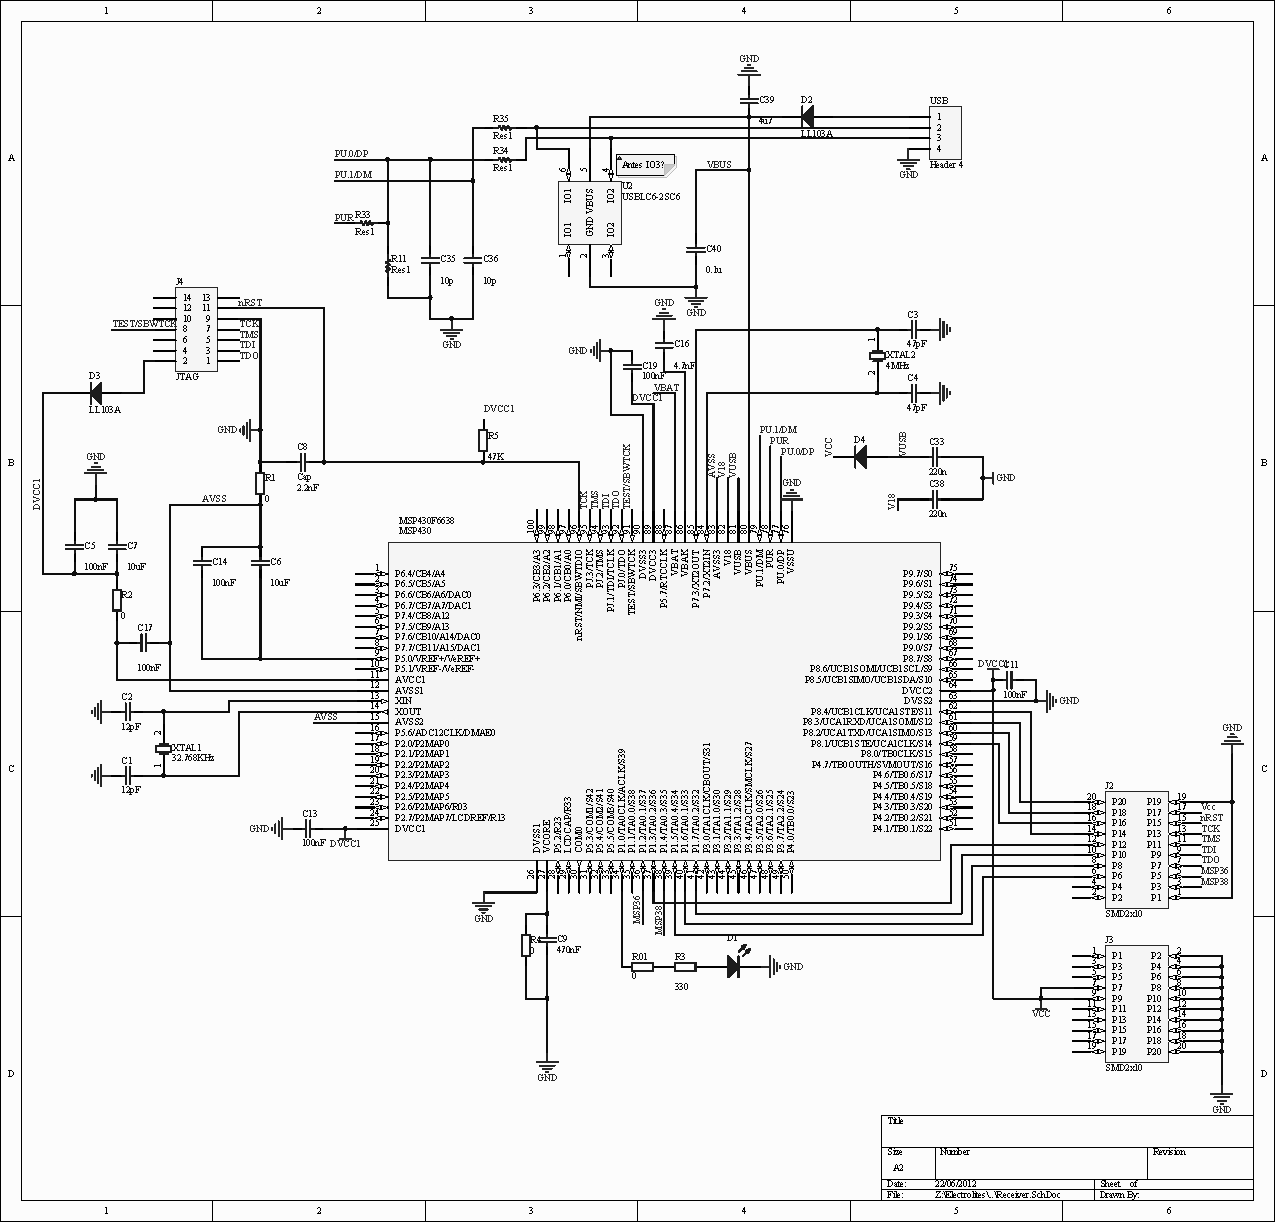
\includegraphics[width=\textwidth,angle=270]{schematic}
\newpage
\section{Printed Circuit Board Design}

\centering
The board design is made in two layers, as follows.\\
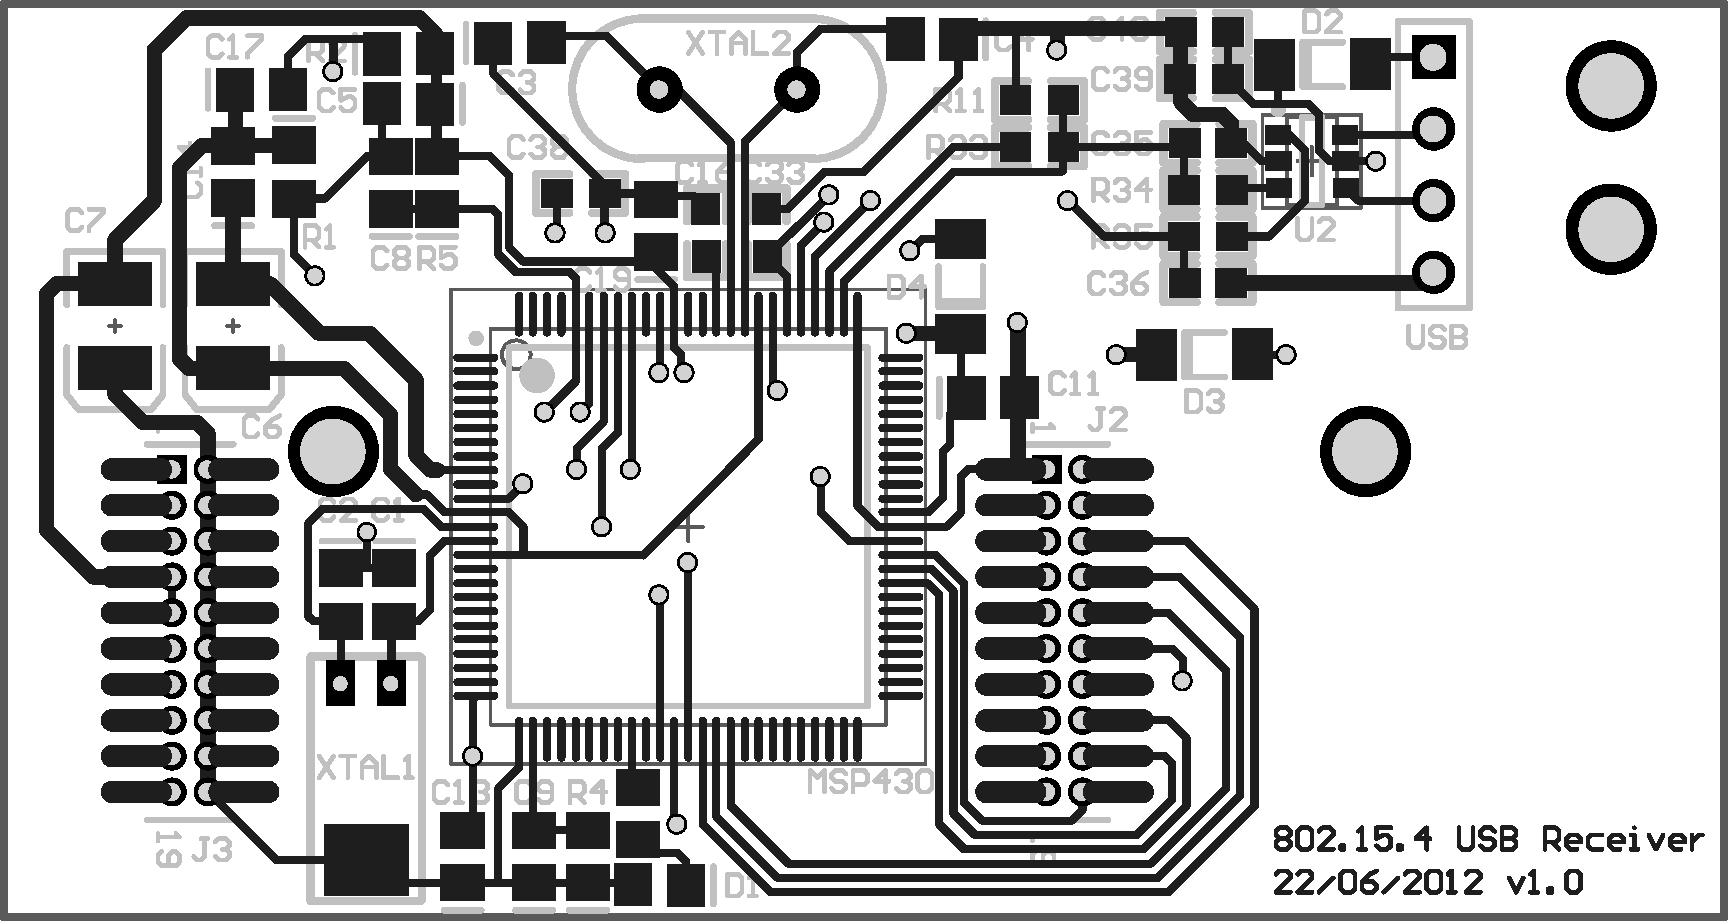
\includegraphics[scale=0.4]{pcb-a}\\
\centering
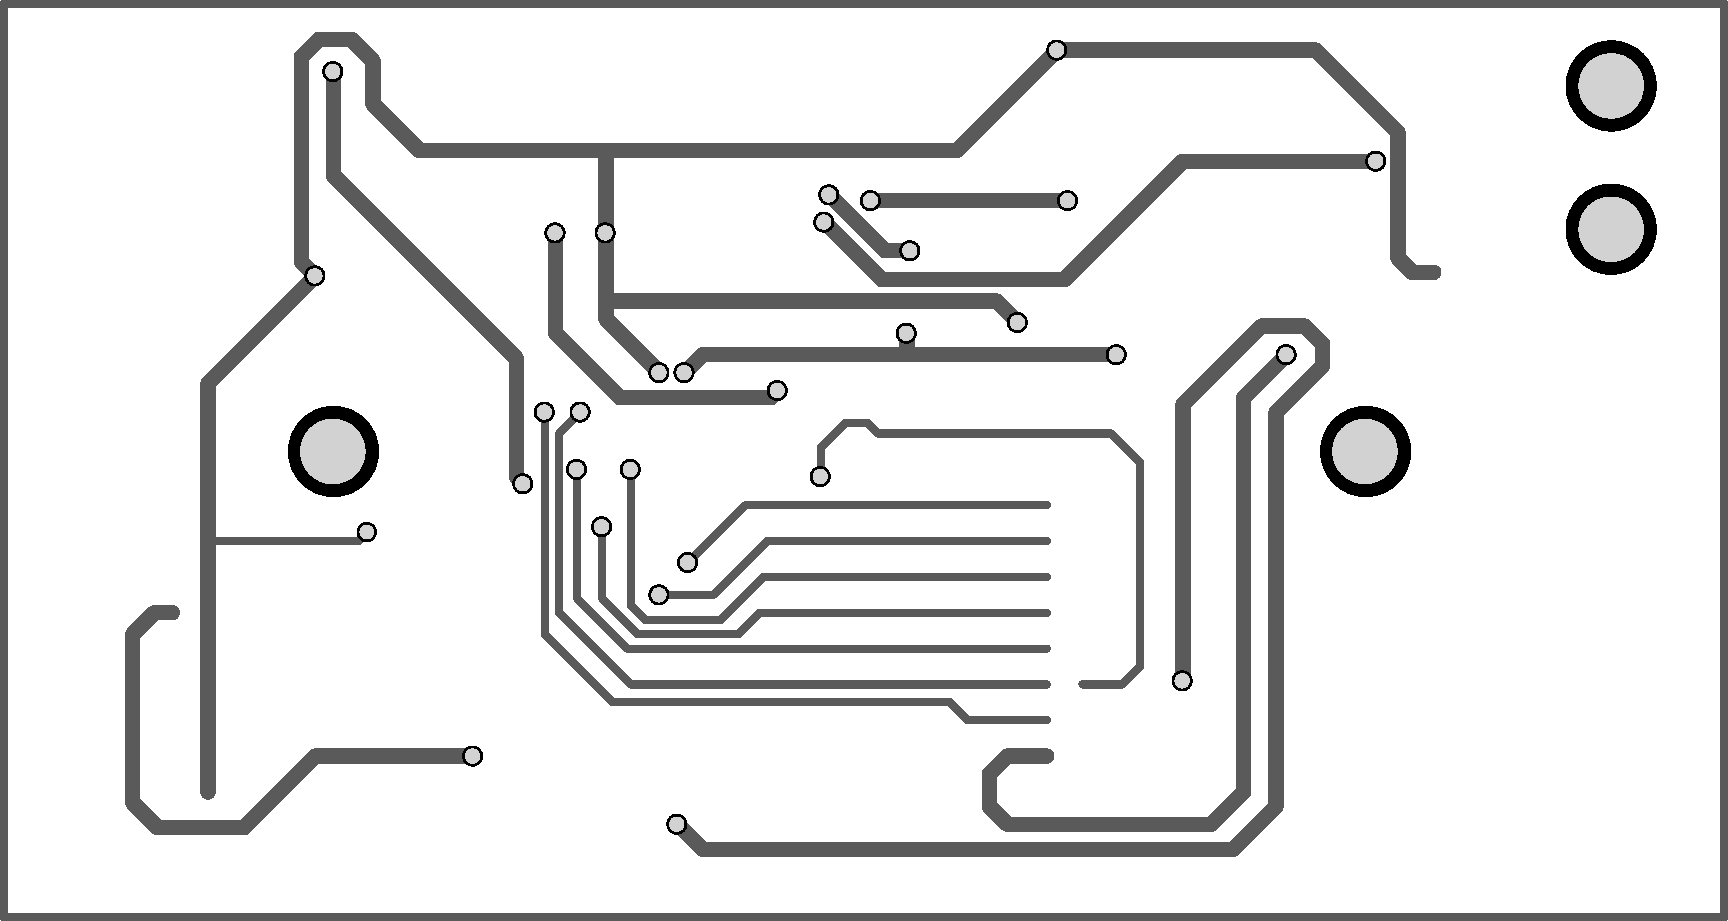
\includegraphics[scale=0.4]{pcb-b}\\

The resulting printed circuit board is as follows.\\

\centering
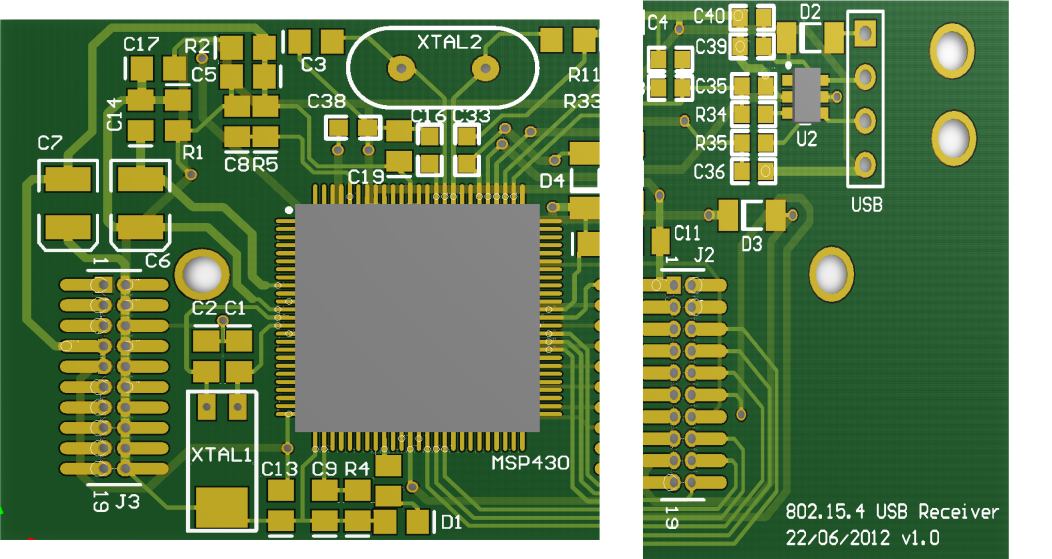
\includegraphics[scale=0.4]{pcb}\\
	\end{appendices}

	% Bibliografía
	\fancyhf{}
	\fancyfoot[RO,LE]{\thepage}
	\renewcommand{\headrulewidth}{0.0pt}
	\renewcommand{\footrulewidth}{0.0pt}
	\begin{thebibliography}{widest-label}

\bibitem{articleTI}
 	Texas Instruments, March 04, 2011\\
 	\emph{TI presents World’s first platform bringing ZigBee to Android smartphones and tablets}.\\
 	\url{http://www.ti.com/ww/in/news_detail/2011/news_detail_20110304.html}\\
%\bibitem{journal:itjq12002}{\it Hyper-Threading Technology},
%Intel Technology Journal,
%Volume 06 Issue 01,
%Published February 14 2002,
%ISSN: 1535766X

%\bibitem{HaNO97} {\it A single-chip multiprocessor},
%L. Hammand, B. A. Nayfeh, \& K. Olukotum,
%IEEE Computer, 30(9):79-85,Sep. 1997.

%\bibitem{libro:lkd}{\it Linux Kernel Development},
%Rovert Love,
%Ed. Sams Publishing, 2004,
%ISBN: 0-672-32512-8

%\bibitem{paper:sched2681}{\it Understanding the Linux 2.6.8.1 CPU Scheduler},\newline
%Josh Aas (\href{mailto:josh@trancesoftware.com}{josh@trancesoftware.com})\newline
%\copyright 2005 Silicon Graphics, Inc. (SGI)\newline
%17th February 2005\newline
%\href{http://josh.trancesoftware.com/linux/}{http://josh.trancesoftware.com/linux/}

\end{thebibliography}


\end{document}
